\chapter{Structural Theory of Coordination Chemistry}
%
\section{Ligand Field Theory}
%
As discussed in \ref{polar}, two singly occupied orbitals with large energy gap tend to form ionic bonds. 
However if one is empty and the other is full, a \emph{dative bond} would form, 
which contributes to various properties of d- and f-bolck elements.
%
\subsection{Sigma Bonding in Octahedral Field}
%
If six ligands, each with one lone pair pointing towards the central atom, form a octahedral configuration around it, 
the ligand orbitals is then of $O_h$ symmetry, 
which can be decomposed into combinations with respect to irreducible representations
by means of SALC (see \ref{salc}).
%
\begin{align*}
	a_{1g}&: \sigma_1 + \sigma_2 + \sigma_3 + \sigma_4 + \sigma_5 + \sigma_6 \\
	t_{1u}&: \sigma_1 - \sigma_3,\quad \sigma_2 - \sigma_4,\quad \sigma_5 - \sigma_6 \\
	e_g&: \sigma_1 - \sigma_2 + \sigma_3 - \sigma_4,\quad 2\sigma_6 + 2\sigma_5 - \sigma_4 - \sigma_3 - \sigma_2 - \sigma_1
\end{align*}
%
As for the central d-block atom, its valence shell $n$d, $(n+1)$s, $(n+1)$p orbitals 
are of $e_g\oplus t_{2g}$, $a_{1g}$ and $t_{1u}$ species respectively. 
Interacting orbitals with the same irrep gives the orbital-energy profile of octahedral complexes.\\ \\
%
However, ligand lone pairs generally have energies a lot lower than metal orbitals, 
causing the six bonding orbitals largely localize on ligands 
while $t_{2g}$ and $e_g^*$ orbitals are almost completely dominated by the central atom.\\ \\
%
This effect can be understood that 12 ligand electrons fill up six ligand-dominated orbitals 
while metal d orbitals \emph{split} into two groups in which the metal electrons then fill.
The energy gap of which is called octahedral \emph{splitting energy}, denoted as $\Delta_O$, 
depends both on ligands and central atom:
%
\begin{itemize}
	\item Ligand: The higher the ligand orbital energy, the smaller the energy gap between ligand and metal d orbitals, 
			thus the greater the interaction energy and greater antibonding elevation.
	\item Metal: Within a same group, the heavier the atom, 
			the wider its d orbitals spread and thus the better interaction between metal and ligand.
\end{itemize}
\ 
\begin{figure}[h]
	\centering
	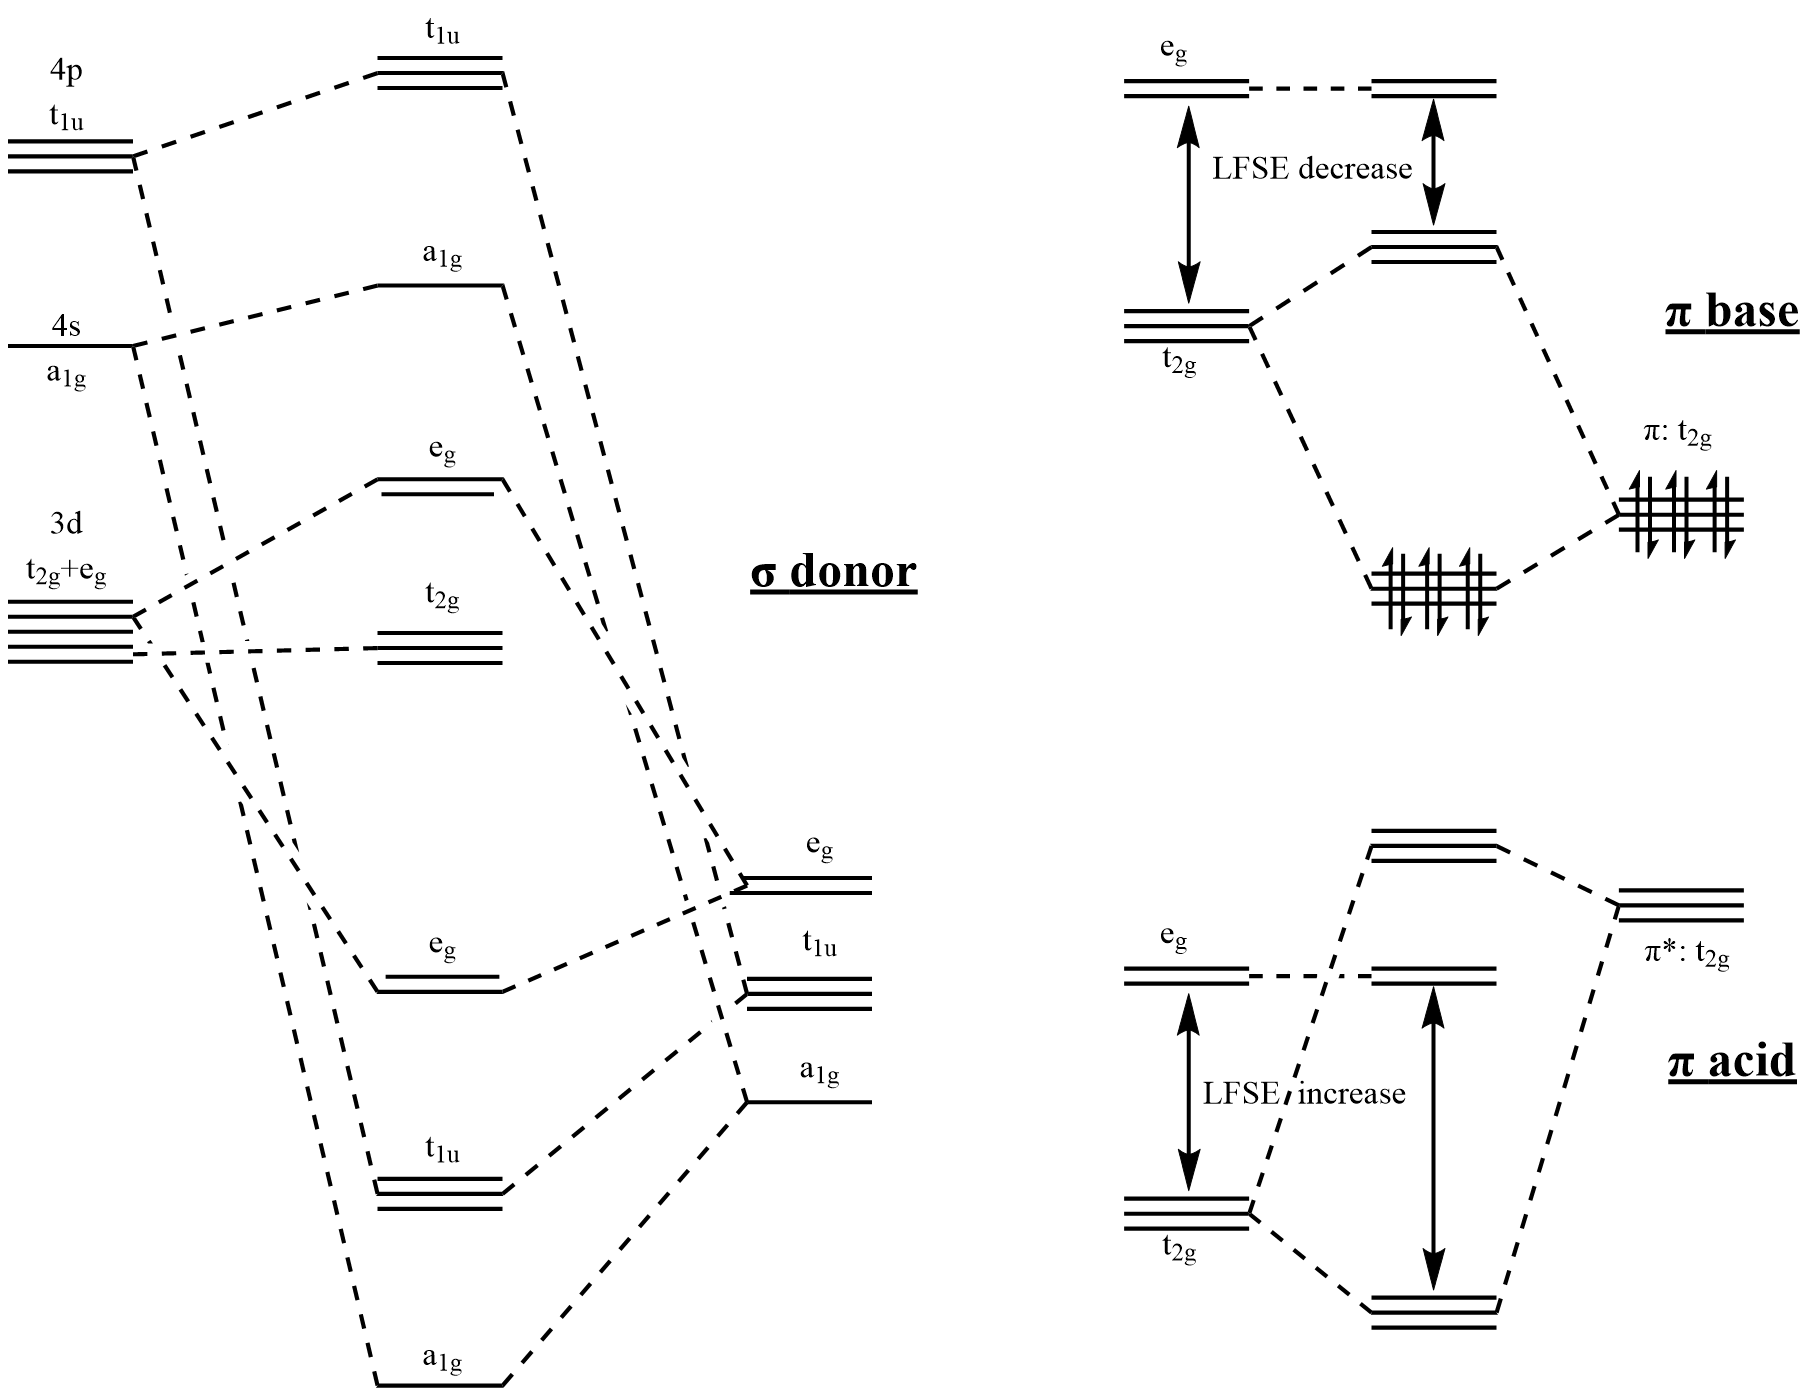
\includegraphics[scale=0.3]{Ch9/lft}
	\caption{Orbital-energy profile of octahedral complexes.}
\end{figure}
%
\subsection{Ligand Field Stabilizing Energy}
%
After all $t_{2g}$ orbitals have been singly occupied, the fourth electron can either:
%
\begin{itemize}
	\item Fill in the upper $e_{g}$ orbitals, which requires it to overcome splitting energy $\Delta_O$, or
	\item Pair up in the $t_{2g}$ orbitals, which requires pairing energy $P$ to counteract electron repulsion.
\end{itemize}
\ 
Therefore for electron configurations $d^4$ through $d^7$, there're two ways to populate orbitals, namely:
%
\begin{itemize}
	\item Weak Field, High Spin: When $\Delta_O<P$, electrons will first singly occupy $e_g$ orbitals then pair up $t_{2g}$ orbitals;
	\item Strong Field, Low Spin: When $\Delta_O>P$, electrons will first pair up $t_{2g}$ orbitals then singly occupy $e_g$ orbitals.
\end{itemize}
%
Because the strong interaction of heavier metals and ligands and small $P$ due to their widespread d orbitals, 
heavy metals largely prefer low spin configurations.
Assuming the energy of d orbitals remain unchanged after splitting, 
the energy reduction after splitting, namely \emph{ligand field stabilizing energy} (LFSE) can then be calculated:
%
\[
	\text{LFSE}=(-\frac{2}{5}n_t+\frac{3}{5}n_e)\Delta_O +nP
\]
%
Where $n_t$ and $n_e$ are numbers of electrons populating $t_{2g}$ and $e_g$ orbitals, 
and $n$ is the number of extra pairs compared to the electronic configuration of quintuple degenerate d orbitals.\\ \\
% 
Knowing the electronic configuration the spin magnetic moment of light atom complexes can then be calculated (see \ref{soc} and \ref{spin1}):
%
\[
	\mu=g_e\gamma_eS=g_e\gamma_e\hbar\sqrt{s(s+1)}
\]
%
For $N$ unpaired electrons the spin quantum number is $N/2$. 
Define Bohr magneton as a scale using $g\approx2$, then:
%
\[
	\mu = \sqrt{N(N+2)}\mu_B, \quad \mu_B = \frac{e\hbar}{2m_e}
\]
%
However when orbital angular momentum participates, situation becomes complicated which is often seen in heavier atoms.
%
\subsection{Ligand Field of Other Symmetries}
%
Utilizing the same approach as we used in octahedral field, a concise conclusion can be obtained that:\\
A set of degenerate orbitals split according to irrep decomposition with respect to its symmetry environment.\\ \\
%
Hence cubic complexes have the same configuration but larger splitting energy than octahedral ones 
due to the same $O_h$ symmetry but more ligands, 
so as square planer and tetragonal bipyramidal (axial distorted octahedron) which are of $D_{4h}$.
%
\subsubsection{Square Planer Complexes}
%
As $d_{x^2-y^2}$ directly points towards the four ligands with the best spacial overlap, 
its energy rise much higher than other d orbitals. 
Therefore leaving it empty is a wise choice, and hence heavy metals with $d^8$ configuration favours this geometrical field. 
%
\subsubsection{Tetrahedral v.s. Octahedral Field}
%
In tetrahedral field, d orbitals split into groups $e$ with lower energy and $t_2$ with higher energy. 
As none of the d orbitals points to ligands, poor spacial overlap results in small $\Delta_T \approx 4/9\cdot \Delta_O$, 
so generally only the case of high spin configuration is considered.\\ \\
%
Since $\text{LFSE}_O$ attains its maximum at $d^3$ and $d^8$ while $\text{LFSE}_T$ begins to drop from $d^2$ and $d^7$, 
$d^3$ and $d^8$ configurations shows a strong preference towards octahedral environment. 
Similar arguments apply to $d^4$ and $d^9$ configuration which also prefers octahedral sites. 
These preferences are shown in figure \ref{LSFEtrend}.\label{preference}\\
%
\begin{figure}[h]
	\centering
	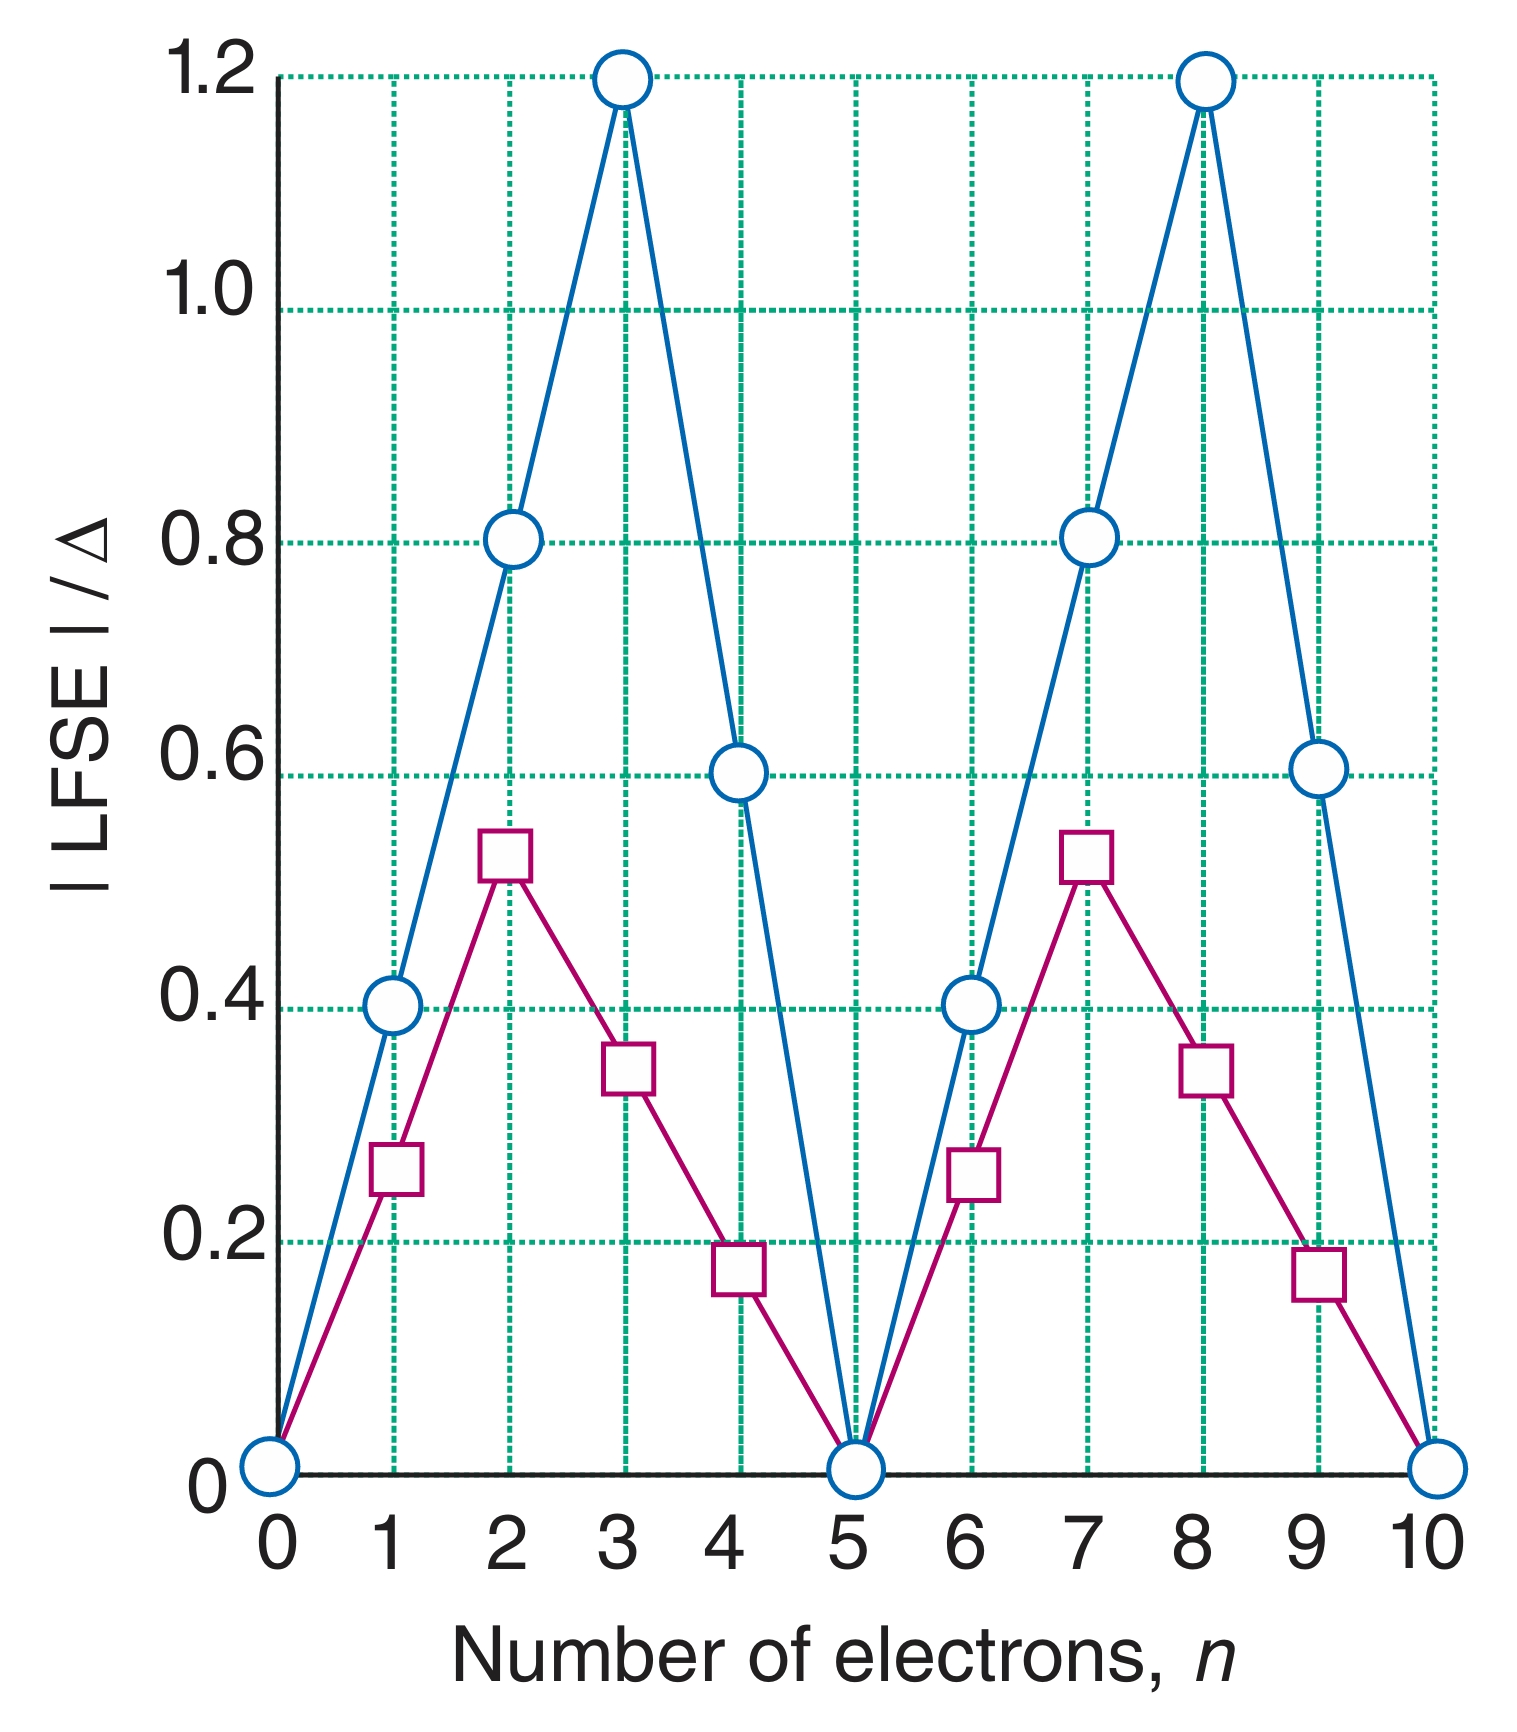
\includegraphics[scale=0.1]{Ch9/octatetrasplit}
	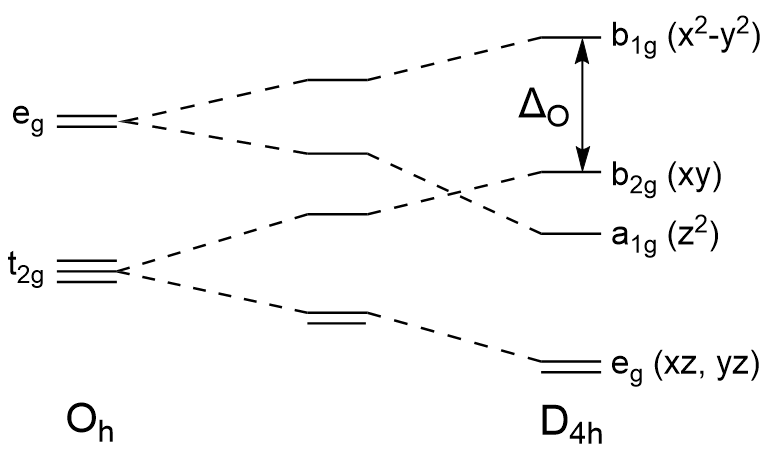
\includegraphics[scale=0.45]{Ch9/jahn-teller}
	\caption{LSFE for $d^n$ configuration in high-spin octahedral and tetrahedral complexes.}
	\label{LSFEtrend}
	\caption{Elongating Jahn-Teller distortion of octahedral complexes}
	\label{jteffect}
\end{figure}
%
\subsection{Jahn-Teller Distortion}
%
Jahn-Teller effect discribes the spontaneous break of symmetry that occurrs in 
asymmetrically populated degenerate orbitals to lower overall energy 
which results in geometrical distortion.\\ \\
%
In octahedral field the $e_g$ orbitals interact strongly with ligands, 
therefore asymmetrically populated (1 or 3 electrons as in HS $d^4$, LS $d^7$ and $d^9$) 
$e_g$ orbitals will distort along $z$ direction. 
%
But it cannot predict the exact distortion mode. 
Since axial elongation with equatorial compression only weakens two bonds while strengthening four, 
whereas the opposite weakens four and strengthens only two, 
\emph{elongated octahedra} ($z$-elongation, $xy$-compression) are more common, 
and in the extreme case where two ligands moves to infinity a square planer field is resulted.
This change is plotted in figure \ref{jteffect}\\
%
Additionally, there exists the \emph{dynamic Jahn-Teller effect}, 
where the complex fluctuates between two distortion directions.\\ \\
In $O_h$, $t_{2g}$ orbitals and in $T_d$ all orbitals do not point directly at ligands, 
so energy changes are less obvious and Jahn-Teller effects are not significant.

%
\subsection{Pi Bonding in Octahedral Field}
%
Besides orbitals that point towards the metal atom, ligands also have orbitals perpendicular to the ligand-metal axis. 
Those orbitals combine and contribute to the $\pi$ bonding of the complex.\\ \\
%
For an octahedral environment, at most 12 orbitals are available for $\pi$ bonds.
However after $\sigma$ bonding, the only orbitals that are ready to form bonds are the metal $t_{2g}$ ones, 
so the ligand orbitals combine and gives a $t_{2g}$ triplet to interact with the metal orbitals.
%
\begin{itemize}
	\item If the $\pi$ orbitals are full and thus lower in energy, the metal orbitals will then become antibonding and be elevated, 
		narrowing the splitting energy. This kind of ligands are named \emph{pi bases};
	\item If the $\pi$ orbitals are empty and thus higher in energy, the metal orbitals will then become bonding and be lowered, 
		widening the splitting energy. This kind of ligands are named \emph{pi acids}.
\end{itemize}
%
Therefore, the \emph{spectrochemical sequence}, which ranks the field strength of ligands, 
is primarily explained by $\pi$ bonding effects:
The stronger the $\pi$ basicity, the weaker the field it create.\\
%
\[
	\text{I}^- < \text{Br}^- < \text{S}^{2-} < \text{SCN}^- < \text{Cl}^- < 
	\text{NO}_3^- < \text{F}^- < \text{OH}^- < \text{C}_2\text{O}_4^{2-} < 
	\text{O}^{2-} < \text{H}_2\text{O} <\]\[ \text{NCS}^- < \text{MeCN} < 
	\text{py} < \text{NH}_3 < \text{en} < \text{bipy} < \text{phen} < 
	\text{NO}_2^- < \text{PPh}_3 < \text{CN}^- < \text{CO}
\]
%
\section{Spectral Properties of Coordination Compounds}
\subsection{d-d Transitions}
%
Although d-d transitions are $g\to g$ transitions which are forbidden according to Laporte selection rules (see \ref{laporte}), 
the complex is continuously vibrating which breaks symmetry and allows this kind of transition to slightly happen.
However tetrahedral complexes have no center of inversion so their color are richer. \\
%
For simple complexes, this is the primary contribution to its color which depends on the splitting energy. 
Therefore the stronger the field ligands create, the more the absorption peak blue-shifts. 
$\pi$ acids not only enhances ligand field splitting but also promotes MLCT, so they often bring vibrant colors.\\ \\
%
Some configurations ($d^5,\ d^{10}$) have no available transition modes as d-d transitions are spin forbidden. 
Those can still take on a faint color due to spin-orbit coupling which will be discussed afterwards.
%
\subsection{Charge Transfer Transitions}
%
Charge transfer transitions are attempted redox reactions, 
which are the transitions between metal-dominated orbitals and ligand dominated orbitals.\\ \\
%
Charge transfer transitions can be laporte allowed, and the change of electron density is large compared to d-d transitions, 
which contributes to a large transition moment.
Therefore it brings the complex an intense absorption peak and rich colors. 
Meanwhile the great electron density shift is significantly affected by the dielectric constant of its environment,
giving rise to a phenomenon called solvatochromism.
%
\subsubsection{Ligand to Metal Charge Transfer}
%
When high energy lone pairs are present on ligands (eg. S, Se) or 
when metals are electron deficient with low-lying empty orbitals, as is often the case in high-valent centers, 
electrons in ligand-dominated orbitals are easily excited into metal-dominated orbitals.
An example is the metalates $[\text{MO}_4^{n-}]$ as in permanganate, chromate and vanadate: 
oxygen lone pairs are exited into empty metal $e$ orbitals.\\
This process can go on to such an extent that the ligand completely donates its electron to the metal, reducing it and decomposes, 
as in metal-oxalate complexes.
%
\subsubsection{Metal to Ligand Charge Transfer}
%
When ligands with low-lying $\pi^*$ orbitals are coordinated to low-valent metals, 
metal electrons get excited and transition to empty ligand orbitals.\\
Strong $\pi$ acids as diimines (2,2'-bpy, 1,10-phen, salen), carbon monoxide and dithialate ions are the ones most prone to have MLCT occur.
%
\begin{figure}[h]
	\centering
	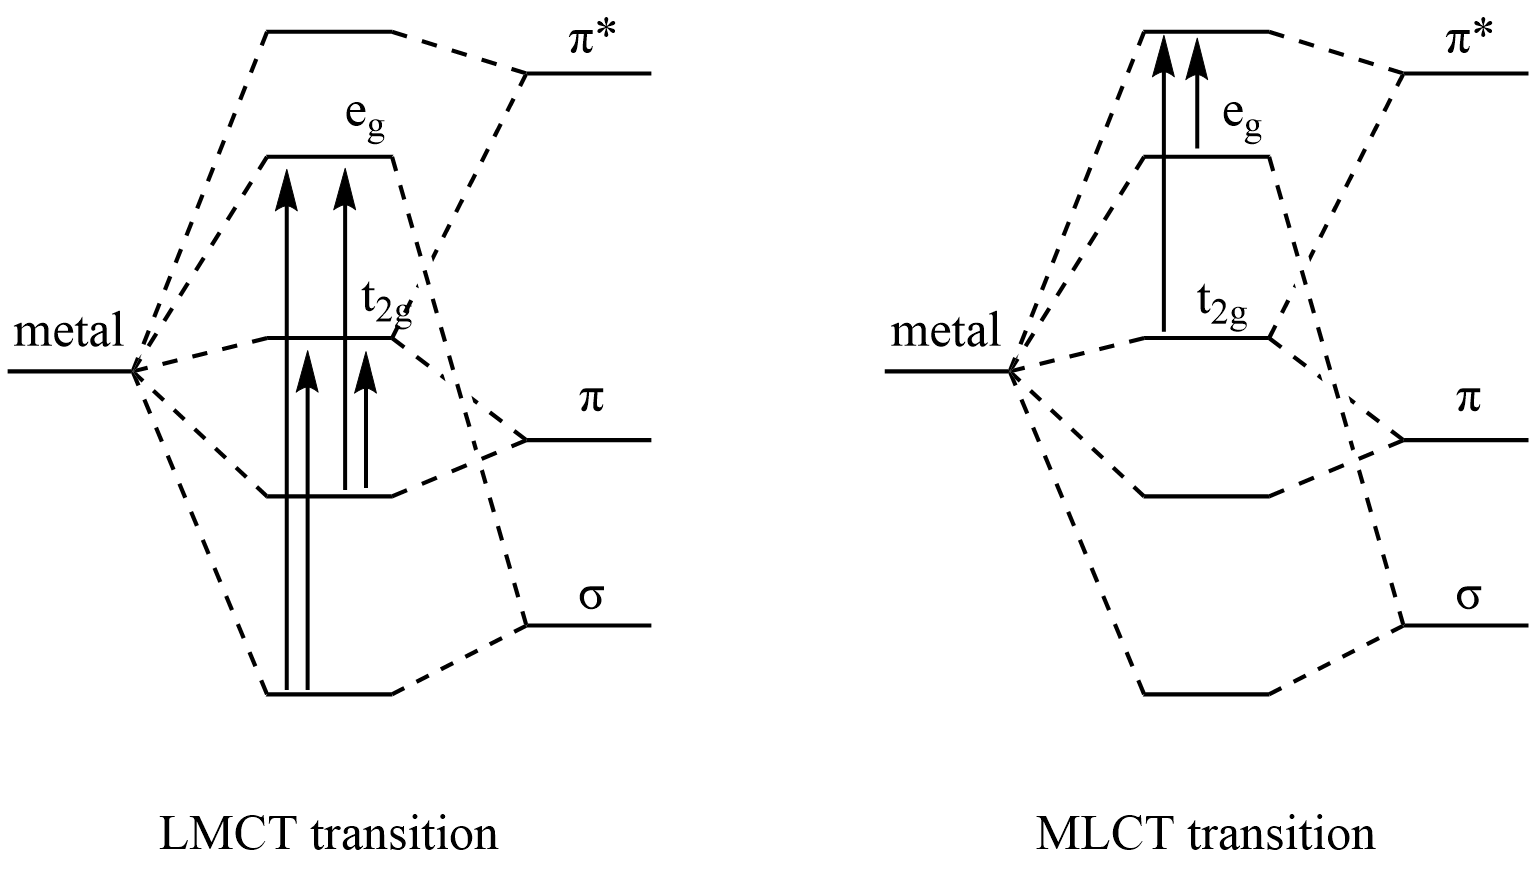
\includegraphics[scale=0.3]{Ch9/ct}
	\caption{Frontier orbital profile of charge transfer transitions}
\end{figure}
%
\section{Spectral Terms of Coordination Compounds}
%
\subsection{Weak Field and Strong Field Limit}\label{split}
%
In free space (spherical symmetry), a specific electronic configuration splits into several spectral terms, 
as discussed in \ref{spectral term}.
When its symmetry environment changes, these terms further splits.\\ \\
%
If the field induced by ligands is weaker than that of electron repulsion, 
those Russell-Saunders atomic spectral terms are still good basis functions and splits according to a previous proof in \ref{molecular term}, 
resulting terms with the same multiplicity.
However in the strong field limit, the field electronic configuration dominates and 
splits into terms with the same electronic configuration.\\ \\
%
Take $d^2$ configuration in octahedral field as an example, and the results are shown in figure \ref{correlation}.\\ \\
Note that when connecting the same molecular terms, intersections of these lines should be minimized. 
This is because two terms of the same symmetry can interact and raise the upper one while lower the lower one. They won't cross and exchange order.
Consequently, these lines will not be absolutly straight. 
As an example, the $T_{1g}(F)$ term and $T_{1g}(P)$ term will interact so that the former bents down and the latter rise up.\\ \\
%
However when $jj$ coupling becomes more significant, the determinating factor is now total angular momentum $J$. 
We discovered that now rotation of $2\pi$ is not an identical operation now, 
so we introduced the \emph{double group} (see \ref{double group}) and perform the exact same operation as the previous example
%
\subsection{Orgel Diagram and Tanabe-Sugano Diagram}
%
Graphing out the term splitting patterns of every electronic configuration 
with their barycenters remain in place gives what so called \emph{Orgel diagram}.
(Technically Orgel diagram only plot out terms with the same multiplicity as the ground state, 
i.e. spectral selection rule permitted states)\\ \\
%
As complement configurations have opposite spectral terms (see \ref{spectral term}, 
and tetrahedral and octahedral environment have opposite energy level order, 
extending the graph in the opposite direction will 
give the Orgel diagram for both octahedral and tetrahedral environment, both $d^n$ and $d^{(10-n)}$ configuration.\\ \\
%
However, the barycenter isn't still. 
Ground state energy decreases as ligand field increases, because metal-ligand interaction increases. 
To solve this we make ground state energy a horizontal line and graph out all spectral terms. 
This kind of plots are named \emph{Tanabe-Sugano diagrams}, after their inventor. 
The vertical line in the middle separates low spin and high spin complexes.
%
\begin{figure}[h]
	\centering
	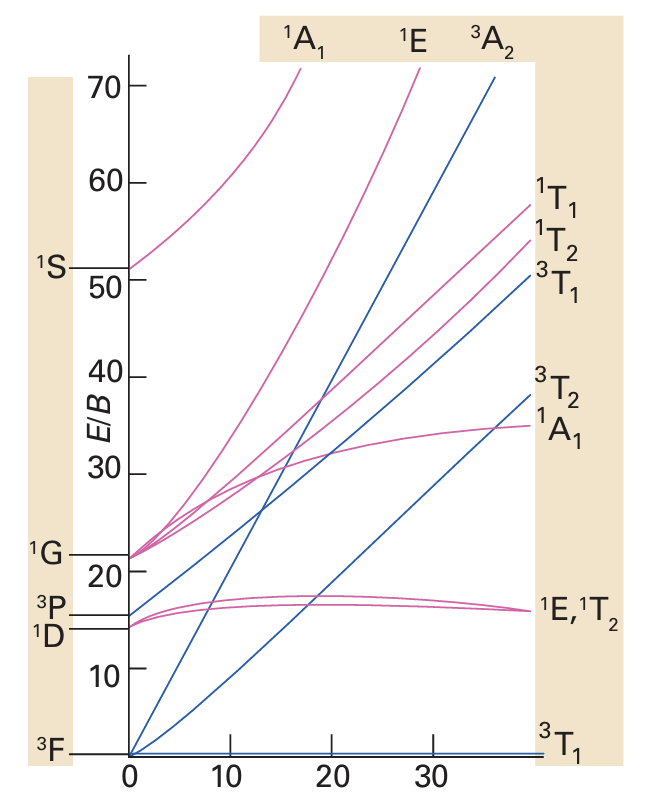
\includegraphics[scale=0.6]{Ch9/tanabe}
	\caption{Tanabe-Sugano diagram for $d^2$ configuration}
\end{figure}
%
\subsection{More Detailed Discussion on d-d Transition}
%
According to the two diagrams we obtained, we can now discuss d-d transition further.
Transitions occur from the ground spectral term to excited terms with the same multiplicity according to spin selection rule.
Specially for $d^1$ configuration, due to Jahn-Teller distortion of the excited $^2T_{2g}\to^2E_g$ $e_g^1$ configuration, 
its absorption peak is relatively intense in d-d transitions.
As for those configurations which have no spin-allowed transitions, spin-orbit coupling will help.
Take terms $^6S$ and $^4G$ of configuration $d^5$ as an example: after spin-orbit coupling, 
%
\[\begin{aligned}
	^6S 	& \to 	^6S_{5/2}\\
	^4G 	& \to 	^4G_{11/2},\ ^4G_{9/2},\ ^4G_{7/2},\ ^4G_{5/2}
\end{aligned}\]
%
Then two states with the same $J$ interact and bring each other components of the other's multiplicity (see \ref{spinflip}),
which then let the transition to slightly occur.
%
\begin{figure}[h]
	\centering
	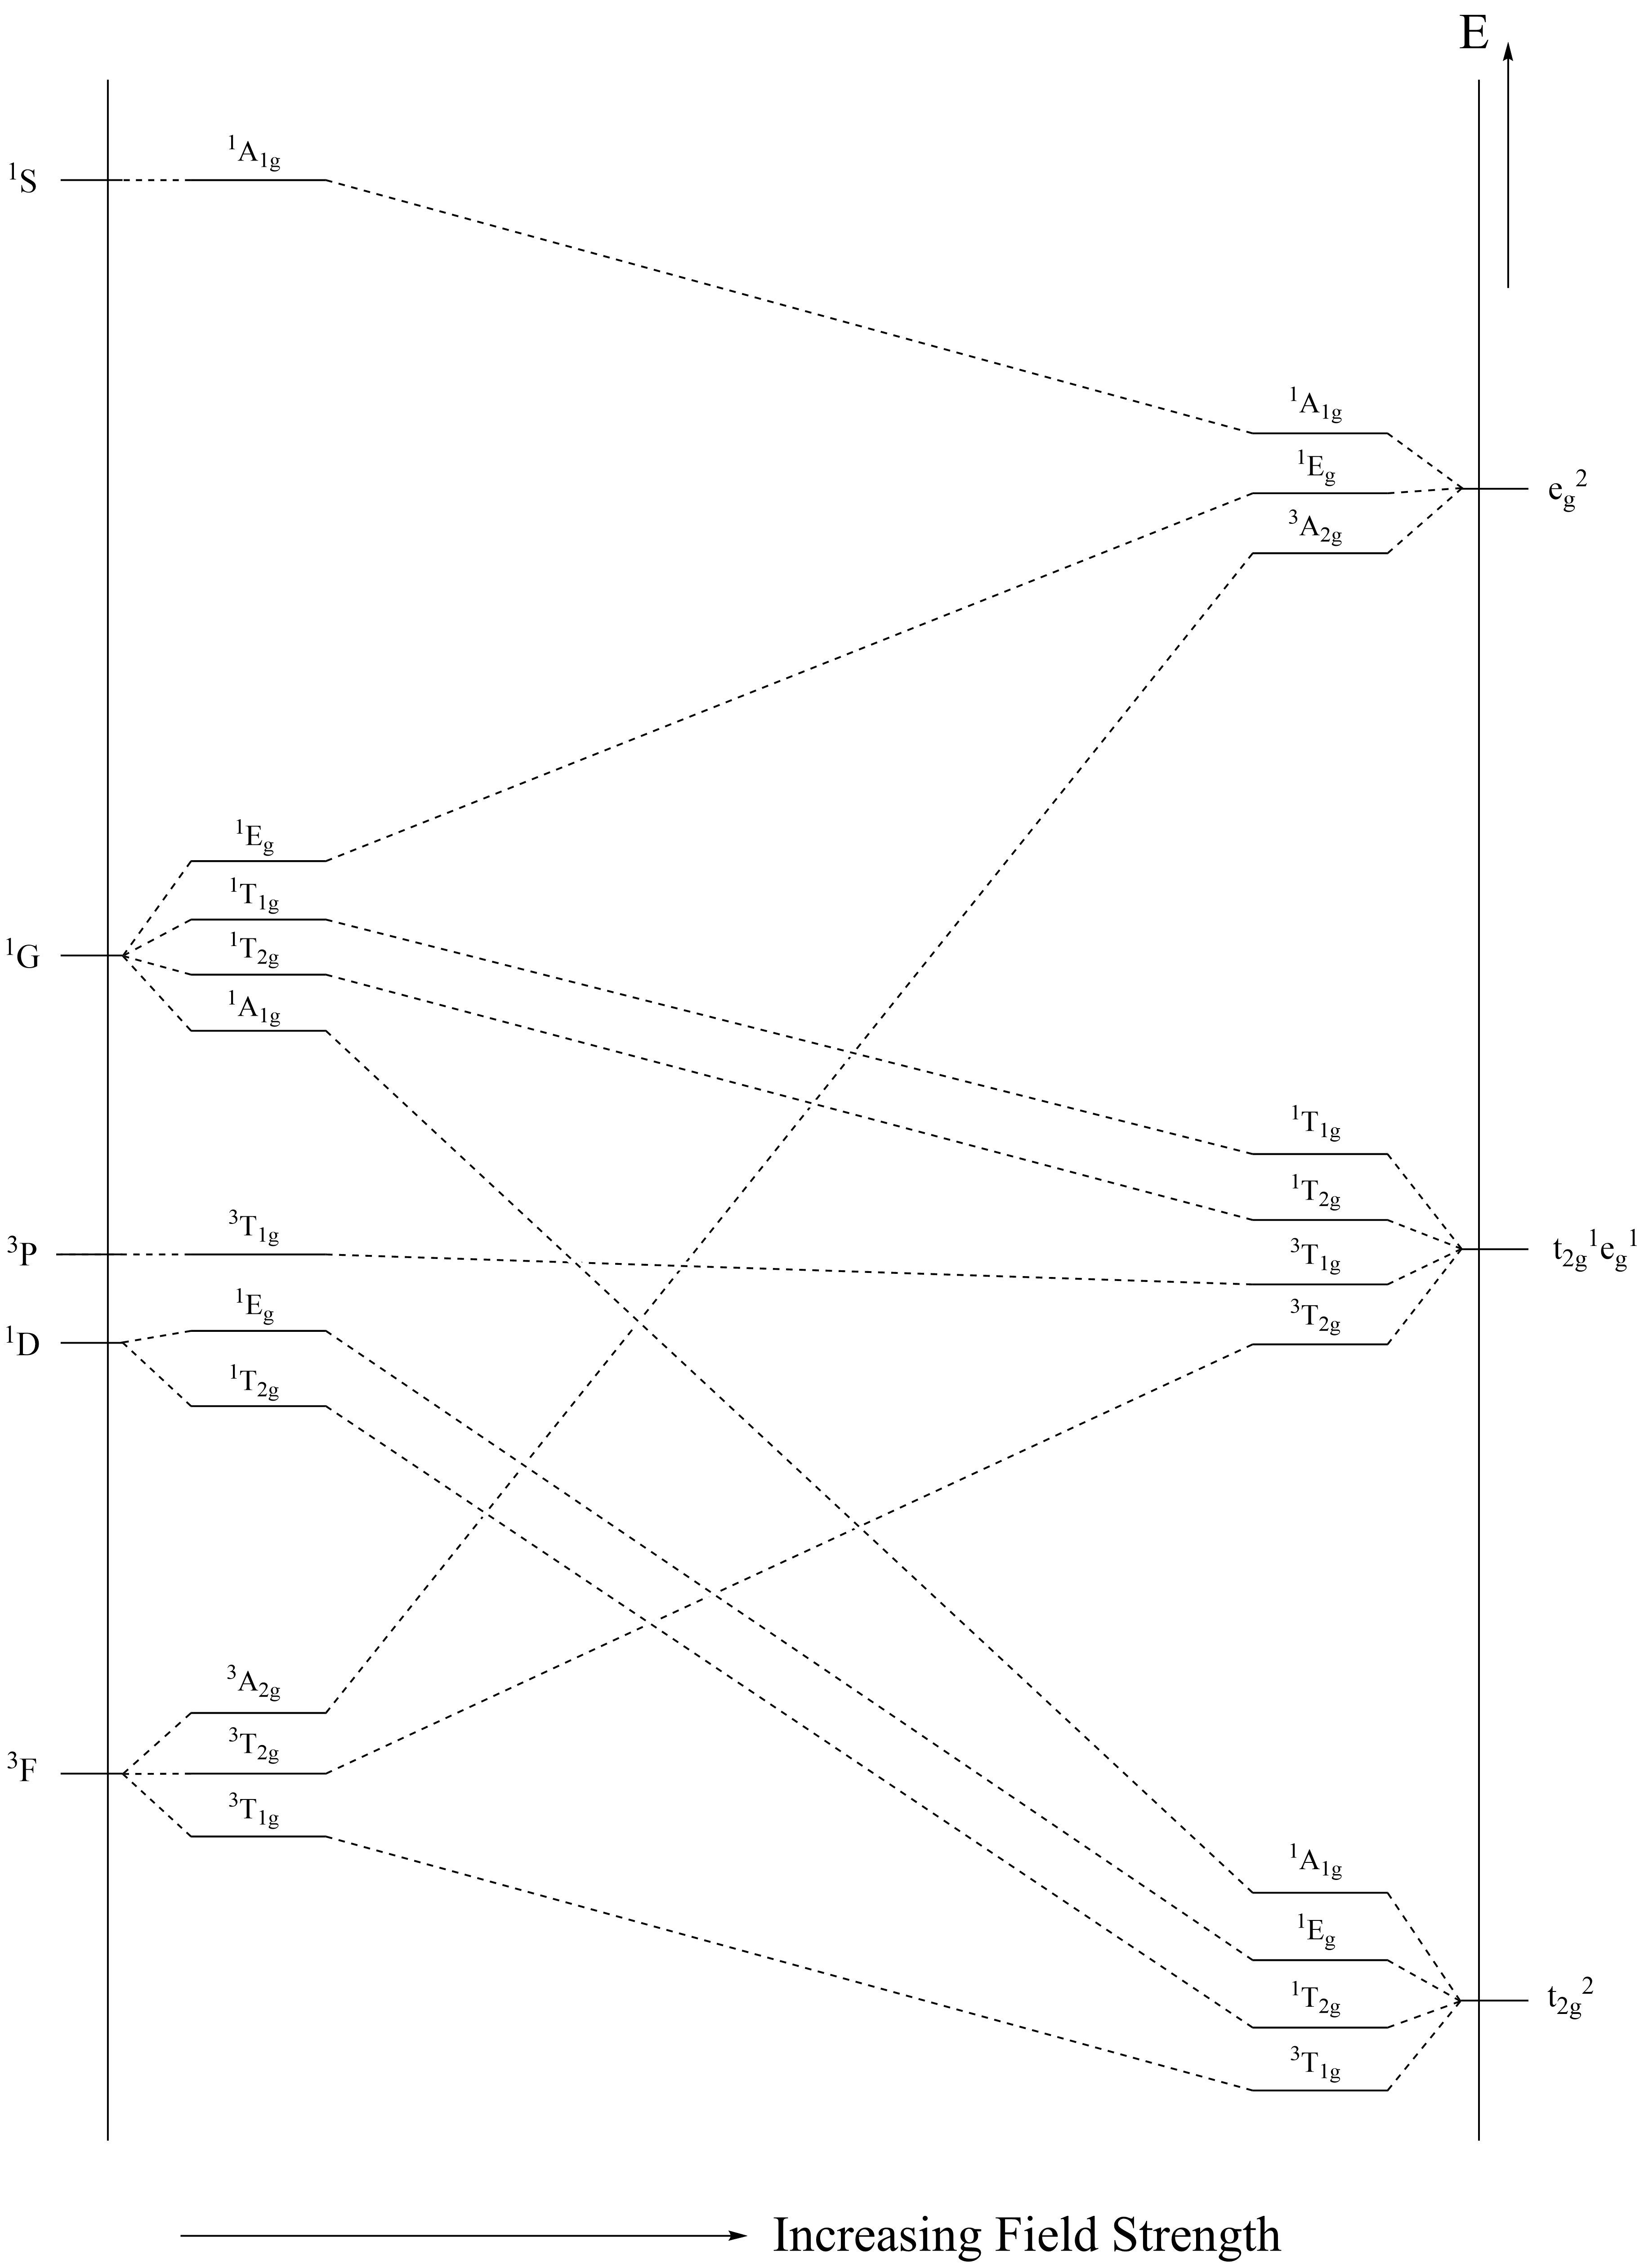
\includegraphics[scale=0.1]{Ch9/complex}
	\caption{Correlation diagram for $d^2$ complexes}
	\label{correlation}
\end{figure}

\section{Organometallics}
%
Organometallic chemistry is the chemistry of compounds containing metal--carbon bonds.
Unlike coordination compounds, which are typically charged with variable d-electron count and soluble in water, 
organometallic compounds are often neutral, possess fixed d-electron count, and are soluble in organic solvents.
Their properties are much closer to organic compounds than inorganic salts, with many having low melting points 
and some even being liquid at room temperature.
%
\subsection{Neutral Ligand Theory of Covalent Bond Classification}
%
The \emph{Covalent Bond Classification} (CBC) method 
provides a systematic framework for classifying ligands in organometallic compounds.
Unlike the donor-pair (ionic) method used in coordination chemistry where ligands are classified as anionic or neutral,
the CBC method treats all ligands as neutral species and categorizes them by the number of electrons 
they contribute to the metal--ligand bond.
%
\subsubsection{Three Basic Ligand Types}
%
Every neutral ligand can be classified into one of three fundamental types based on the number of electrons 
its orbital contributes to the metal--ligand bond. 
One ligand molecule can have more than one orbital participated in coordination, 
and each of these orbitals is assigned with one of the three letters below.
%
\begin{itemize}
	\item \textbf{L-type}: A neutral ligand orbital that donates both electrons of a lone pair to the metal.
	\item \textbf{X-type}: A neutral ligand orbital that contributes one electron to the metal--ligand bond, 
		with the other electron originating from the metal.
	\item \textbf{Z-type}: A neutral ligand orbital that accepts a pair of electrons from the metal.
\end{itemize}
%
A complex containing $l$ L-type, $x$ X-type, and $z$ Z-type ligands is classified as $[\text{ML}_l\text{X}_x\text{Z}_z]$.
%
\begin{figure}[h]
	\centering
	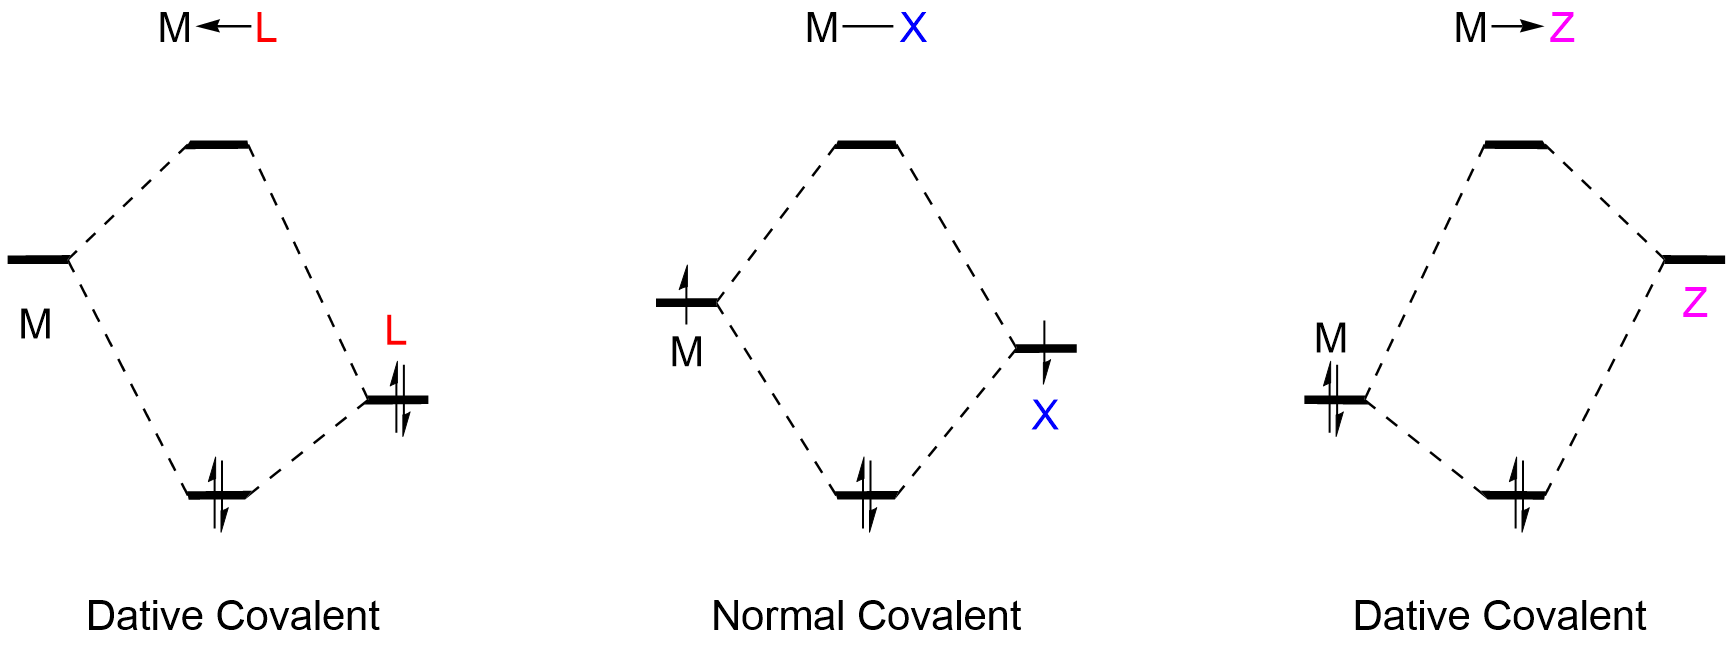
\includegraphics[scale=0.2]{Ch9/cbc}
	\caption{Orbital profile of three ligand types}
\end{figure}\\
%
However, as Z-type ligands do not contribute electrons to the metal center, orbitals that account for Z ligands, 
primarily those low antibonding orbitals, are often omitted in bookkeeping even though they do take part in coordination.
Some exceptions are that when degenerate orbitals are partially occupied, the vacant ones will be denoted as Z.
For instance, ligands shown in figure \ref{cbcligand} are assigned L, L$_2$X, L$_3$, L$_3$XZ respectively. 
%
\begin{figure}[h]
	\centering
	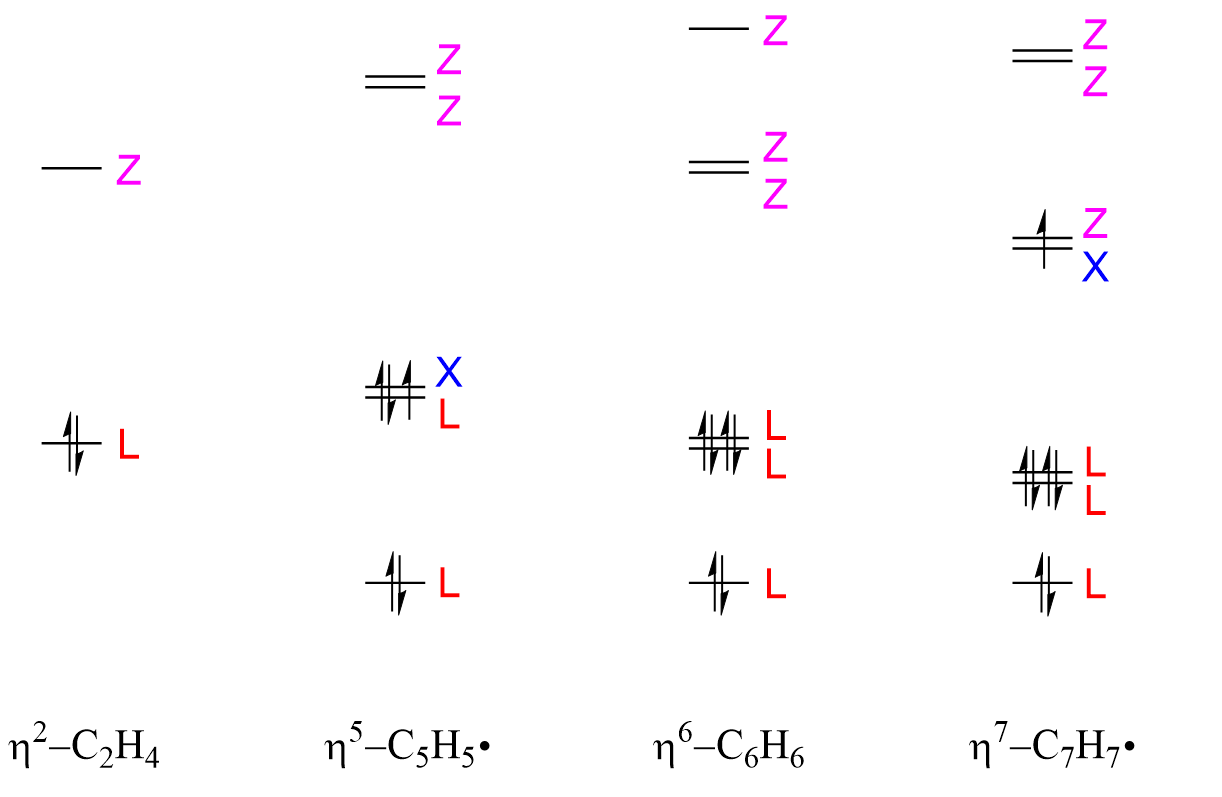
\includegraphics[scale=0.25]{Ch9/cbcligand}
	\caption{Orbital profile and ligand type assignment of some ligands}
	\label{cbcligand}
\end{figure}
%
\subsubsection{Electron Counting and the 18-Electron Rule}
%
The total valence electron count of a complex is obtained by summing the metal's valence electrons  
with the electrons contributed by each ligand.
Most stable d-block organometallic compounds obey the \emph{18-electron rule}, 
having a total of 18 valence electrons around the metal center.
This corresponds to the noble gas configuration where one $s$, five $d$, and three $p$ orbitals are all doubly occupied,
while 16-electron complex are also common.\\ \\
Steric factors may restrict the number of ligands that can bond to a metal atom, 
and stabilize compounds with lower electron counts than might have been expected.
Unusual electron configurations are common on the left of the d block, where the metal 
atoms have fewer electrons, and it is often not possible to crowd enough ligands around 
the atom to bring the electron count up to 16 or 18.
%
\subsection{Sigma Complexes}
%
Alkyl, aryl, and hydride ligands bound through a single M--C or M--H $\sigma$ bond
are classified as X-type in the CBC framework:
the ligand radical contributes one electron and the metal contributes the other.
These \emph{$\sigma$ complexes} are central to organometallic reactivity
because the M--C $\sigma$ bond can be formed, transformed, and broken
through a small set of fundamental reactions.
%
\subsubsection{Oxidative Addition and Reductive Elimination}
%
\emph{Oxidative addition} is the process in which a metal center inserts into a covalent bond A--B,
increasing its oxidation state and electron count each by two:
%
\[
	\text{M}^{(n)} + \text{A--B} \longrightarrow \text{M}^{(n+2)}(\text{A})(\text{B})
\]
%
The reverse is \emph{reductive elimination}, in which two cis ligands couple and depart as a neutral molecule,
lowering both the oxidation state and electron count by two.
Together they form the backbone of catalytic cycles:
oxidative addition activates an otherwise inert substrate, and reductive elimination releases the product.\\ \\
%
The stereochemistry of oxidative addition highly depends on mechanism.
For addition to weakly polarized bonds as H$_2$, C--H and C--C, 
a concerted addition occurrs with retention of stereochemistry, 
while for highly polarized C--X bonds with a fairly good leaving group, 
the addition undergoes with a S$_\text{N}$2-type mechanism with inversion.
%
\subsubsection{Migratory Insertion and $\beta$-Hydride Elimination}
%
\emph{Migratory insertion} is the intramolecular migration of an X-type ligand (alkyl, hydride)
onto a cis-coordinated L-type $\pi$ ligand (CO, alkene), producing a new X-type ligand:
%
\[
	\text{M--R} + \text{CO} \longrightarrow \text{M--C(=O)R}
\]
%
The migrating group retains its stereochemistry at carbon,
making insertion a key step in hydroformylation and polymerization.
The microscopic reverse, \emph{extrusion}, regenerates the starting fragments.\\ \\
%
\emph{$\beta$-Hydride elimination} is the most common decomposition pathway of transition-metal alkyls.
A hydrogen on the $\beta$-carbon transfers to the metal with its electron pair,
generating a metal hydride and a coordinated alkene:
%
\[
	\text{M--CH}_2\text{CH}_2\text{R} \longrightarrow \text{M--H}(\eta^2\text{-CH}_2\text{=CHR})
\]
%
This requires a vacant site \emph{cis} to the alkyl and at least one $\beta$-hydrogen.
Alkyls lacking $\beta$-hydrogens (neopentyl, benzyl, trimethylsilylmethyl) are therefore much more robust
and are preferred when a persistent M--C bond is needed.
%
\subsection{Pi Complexes with Carbonyl and Analogues}
%
\subsubsection{The Synergic Bonding Model}
%
Carbon monoxide is the archetypal organometallic ligand. 
Due to $sp$ mixing and the low-lying atomic orbital of O compared to C, 
the HOMO and LUMO of CO molecular orbital, as shown in figure \ref{como}, 
exhibits large coefficient on C, which makes the C end both nucleophilic and electrophilic, 
enabling its unique coordination behavior described by the \emph{Dewar--Chatt--Duncanson} synergic model with two components:
%
\begin{itemize}
	\item \textbf{$\sigma$ donation}: The carbon lone pair donates into an empty metal orbital (L-type).
	\item \textbf{$\pi$ back-donation}: Filled metal $d$ orbitals donate into the CO $\pi^*$ antibonding orbital.
\end{itemize}
%
\begin{figure}
\centering
\begin{subfigure}[c]{0.4\textwidth}
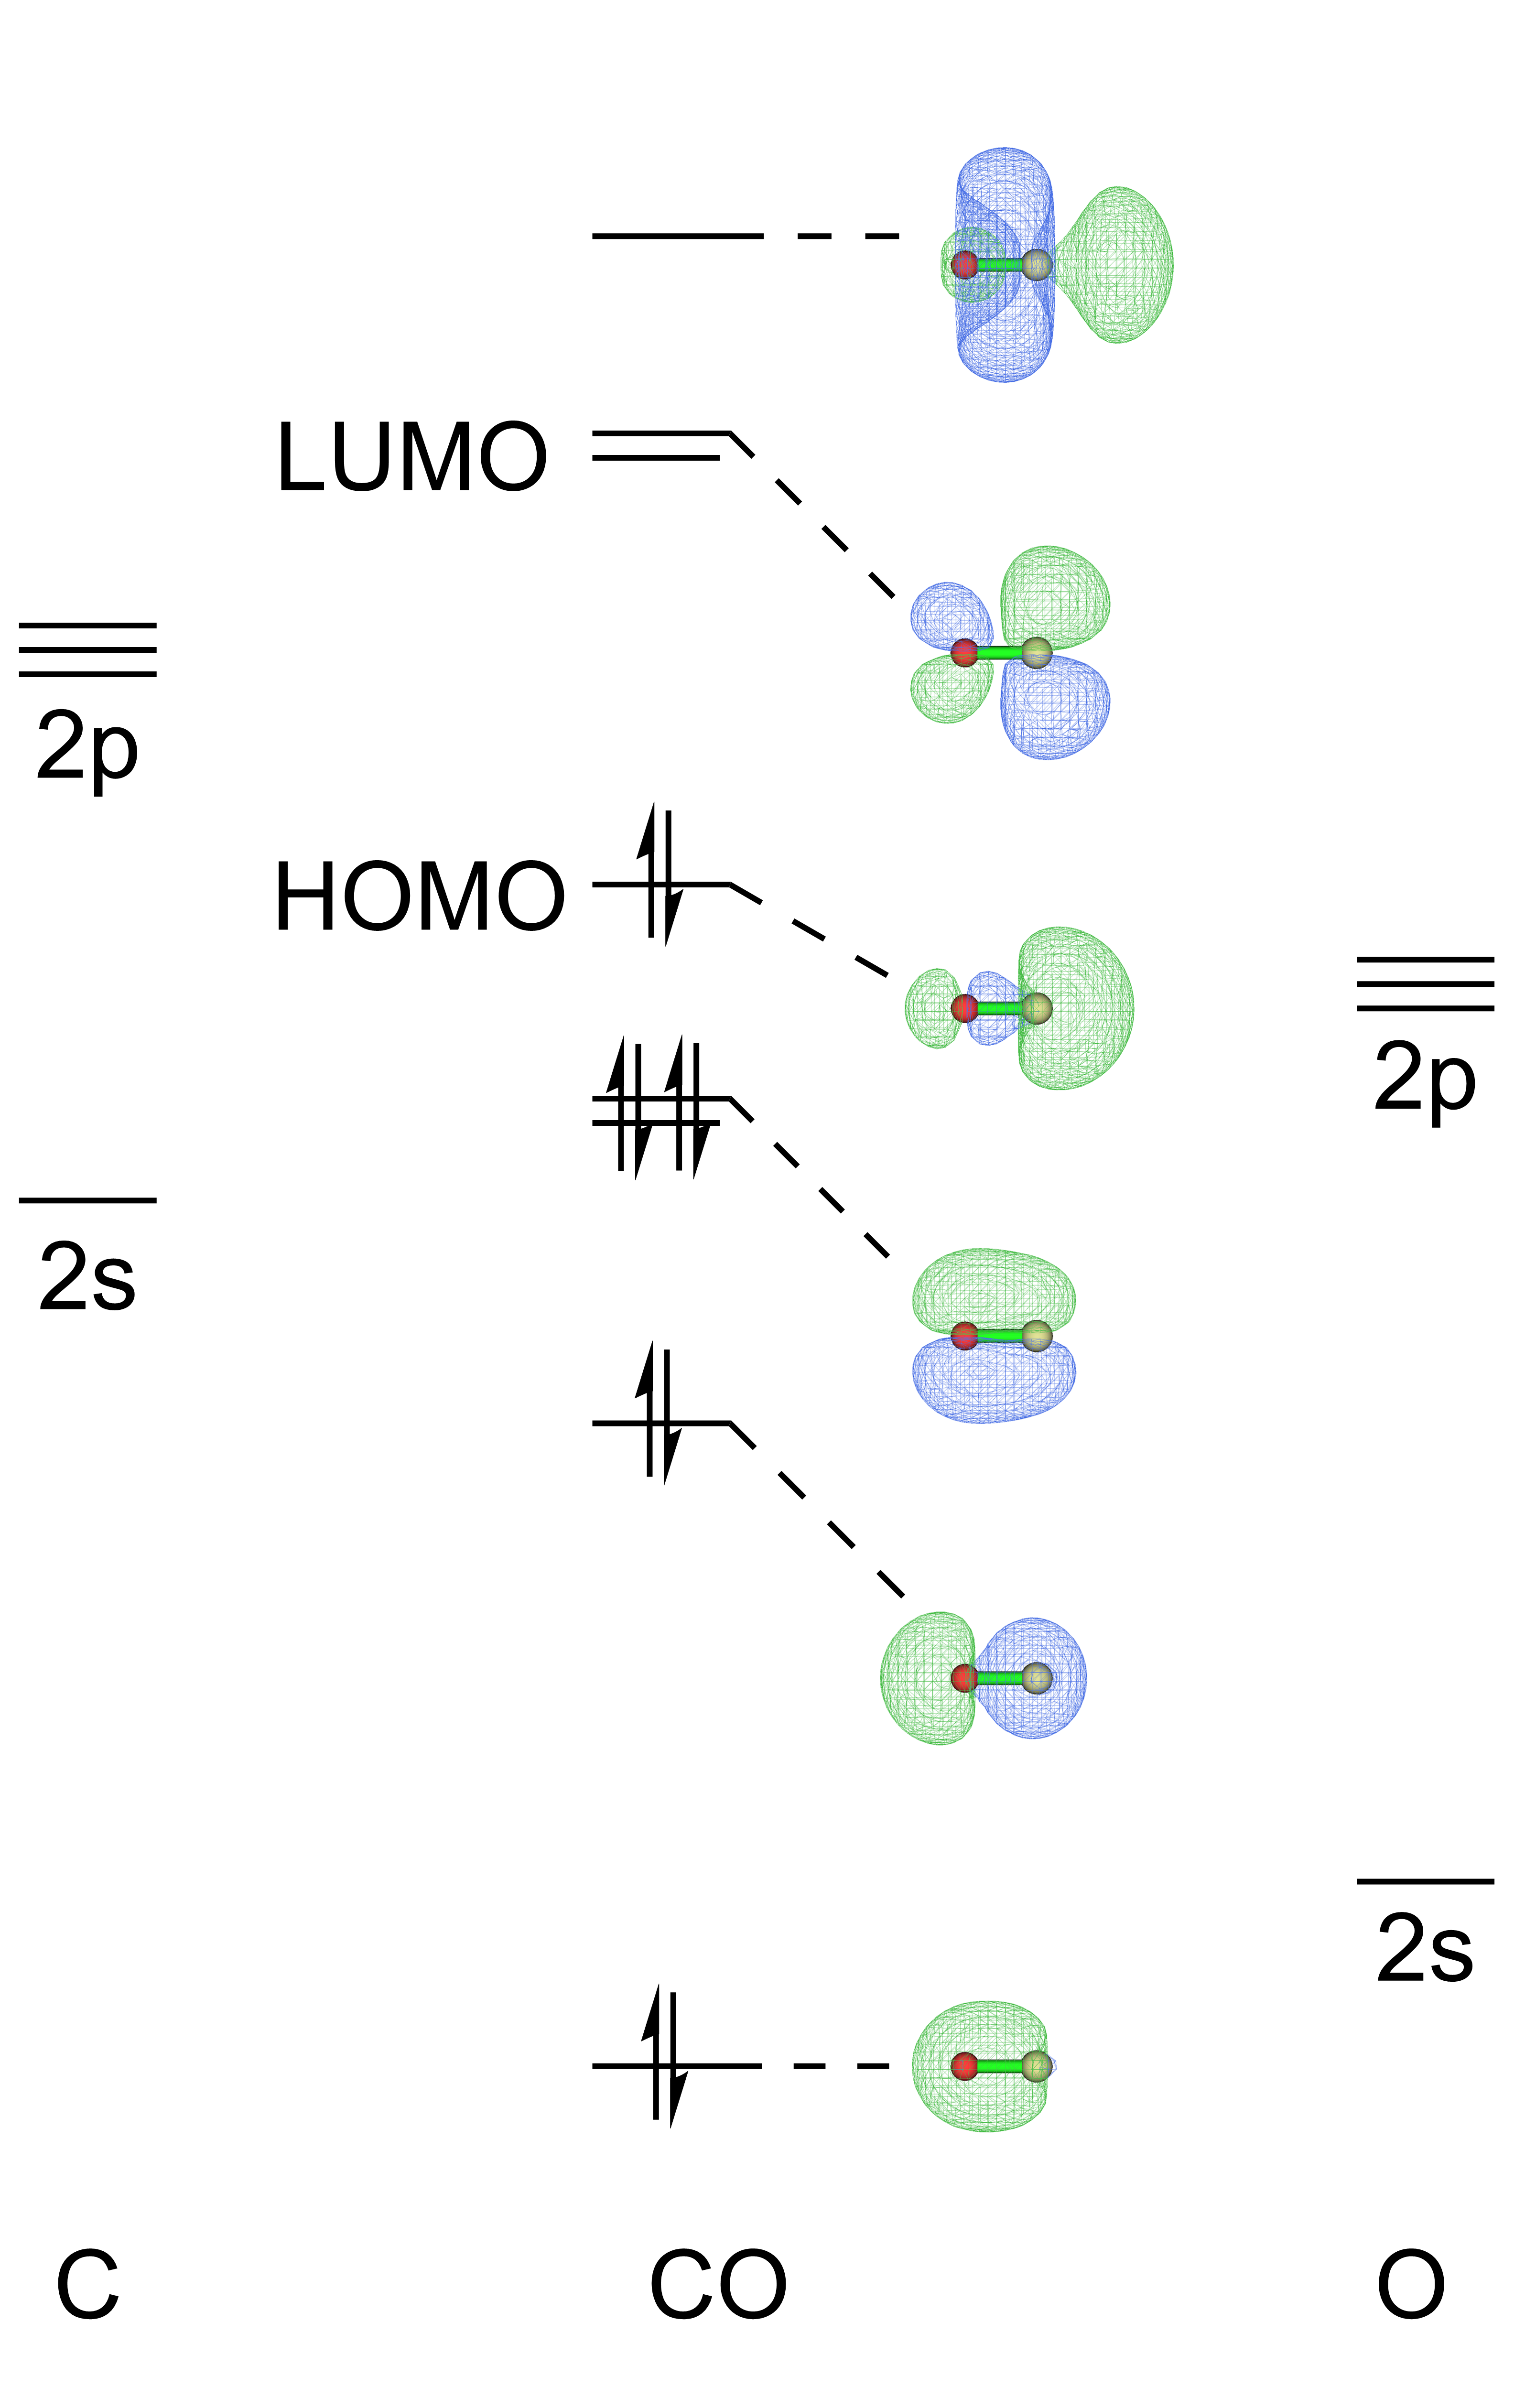
\includegraphics[scale=0.06]{Ch9/CO_MO}
\end{subfigure}
\quad
\begin{subfigure}[c]{0.4\textwidth}
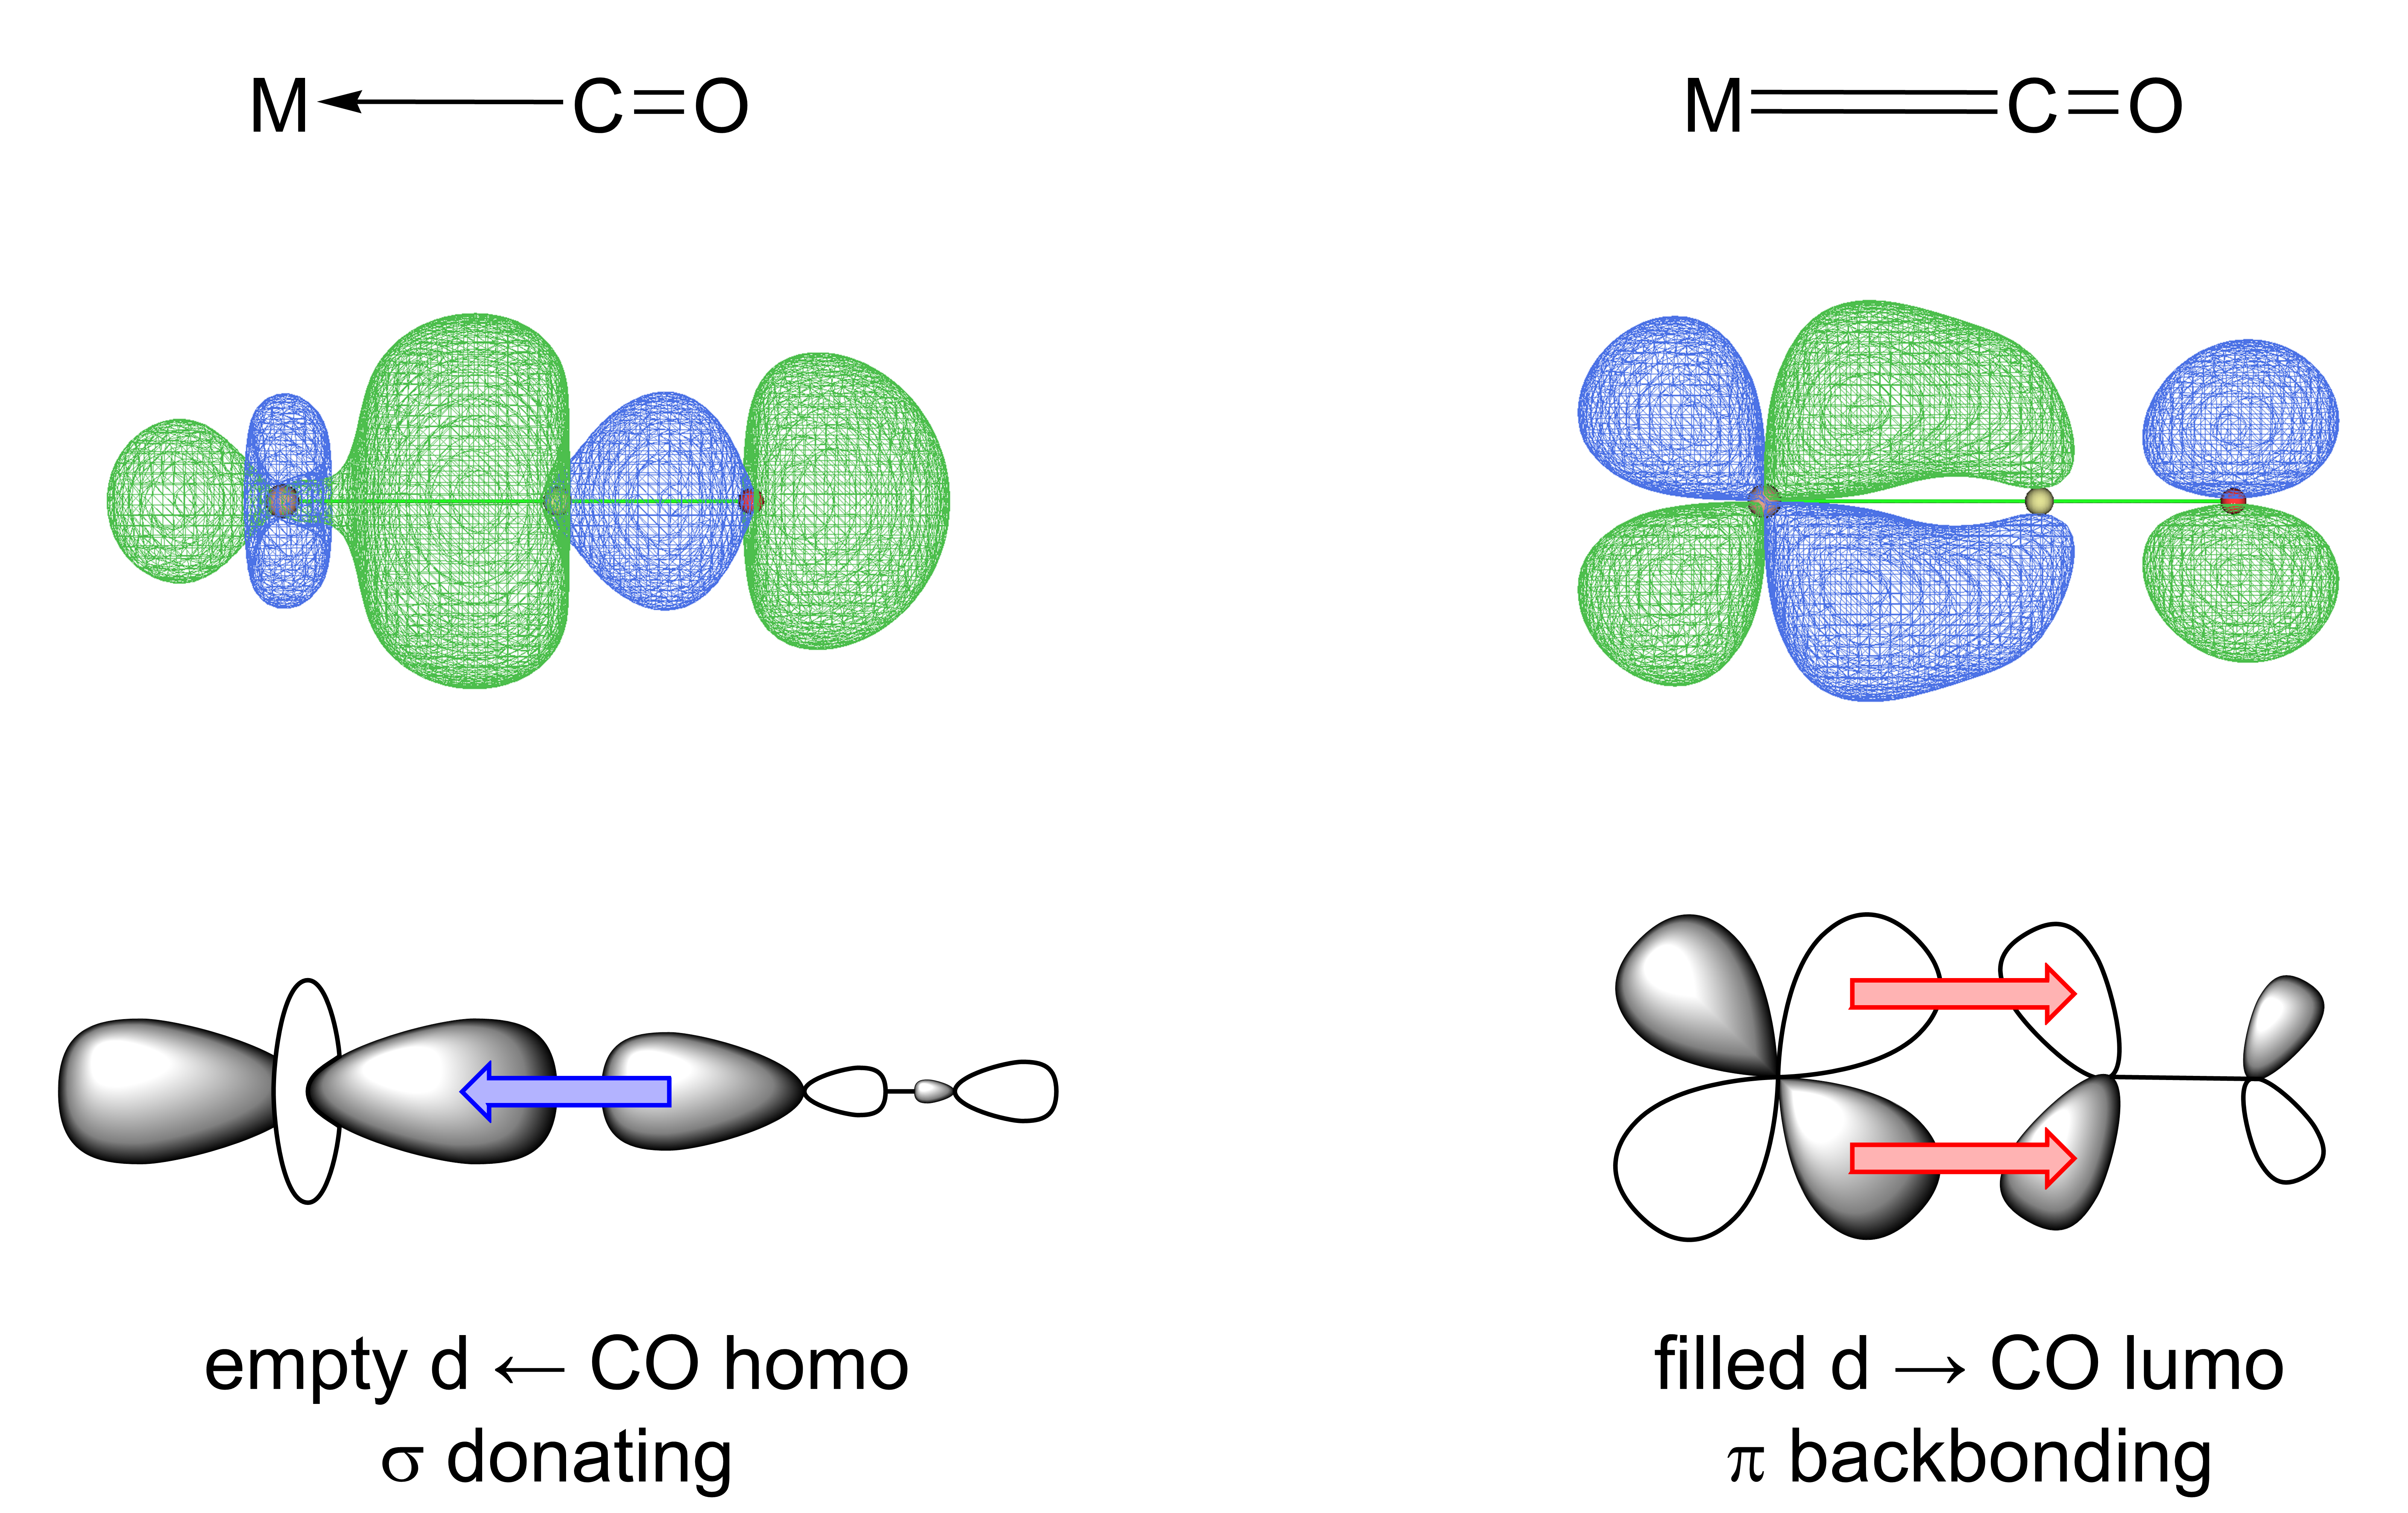
\includegraphics[scale=0.04]{Ch9/MCO}
\end{subfigure}
\caption{Orbital interaction between carbonyl and d-metal}
\label{como}
\end{figure}
%
The two effects reinforce each other:
stronger $\sigma$ donation enriches the metal, enhancing $\pi$ back-donation,
which strengthens M--C but weakens C--O.
The resulting red-shift of $\nu_{\text{CO}}$ relative to free CO (2143 cm$^{-1}$)
makes IR spectroscopy a direct probe of electron density at the metal.
%
In polynuclear complexes CO can bridge multiple metals ranging from $\mu_1$ to $\mu_3$ with 
progressive red-shift reflects increasing $\pi^*$ population as more metals donate into CO.
Figure \ref{comu} shows this trend.\\
%
\begin{figure}[h]
\centering
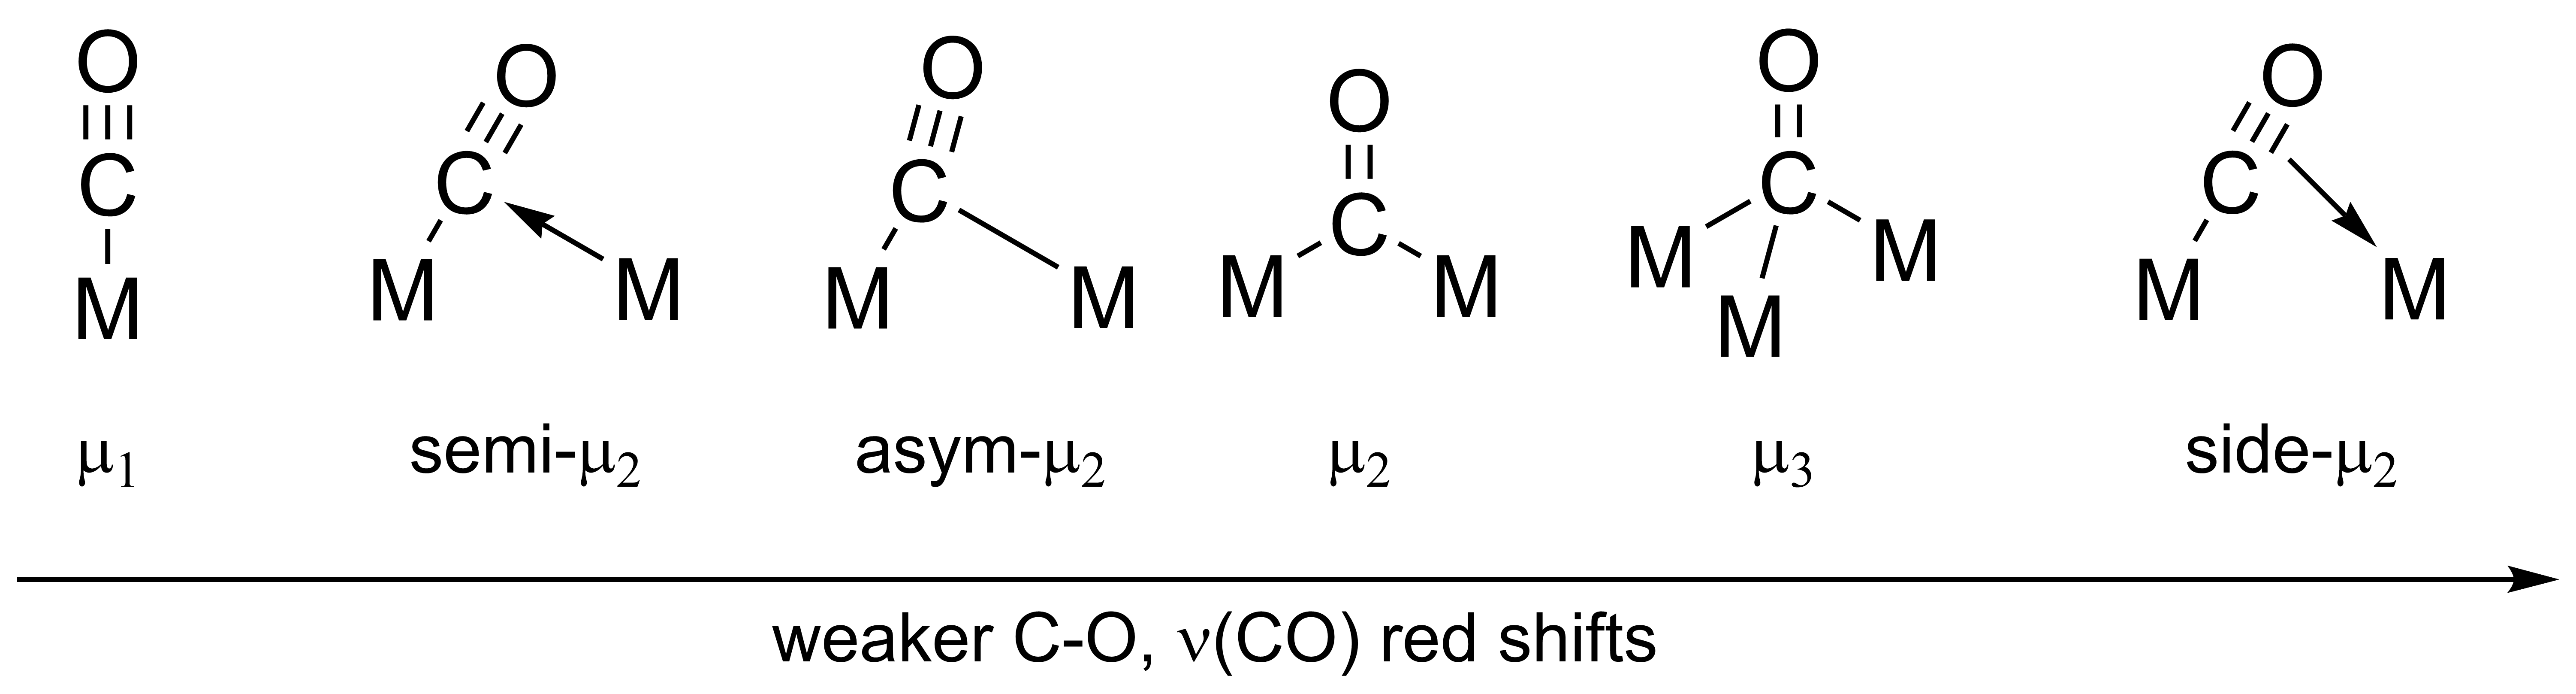
\includegraphics[scale=0.06]{Ch9/comu}
\caption{Red shift of bridging carbonyl}
\label{comu}
\end{figure}\\
%
Among these coordination modes, 
semi-brigding carbonyl forms when one metal center only backdonates without accepting $\sigma$ donation (e.g. figure \ref{semiCO}), 
and side-bridging carbonyl uses its C--O $\pi$ bonding orbital to coordinate with the second metal center.
%
\begin{figure}[h]
\centering
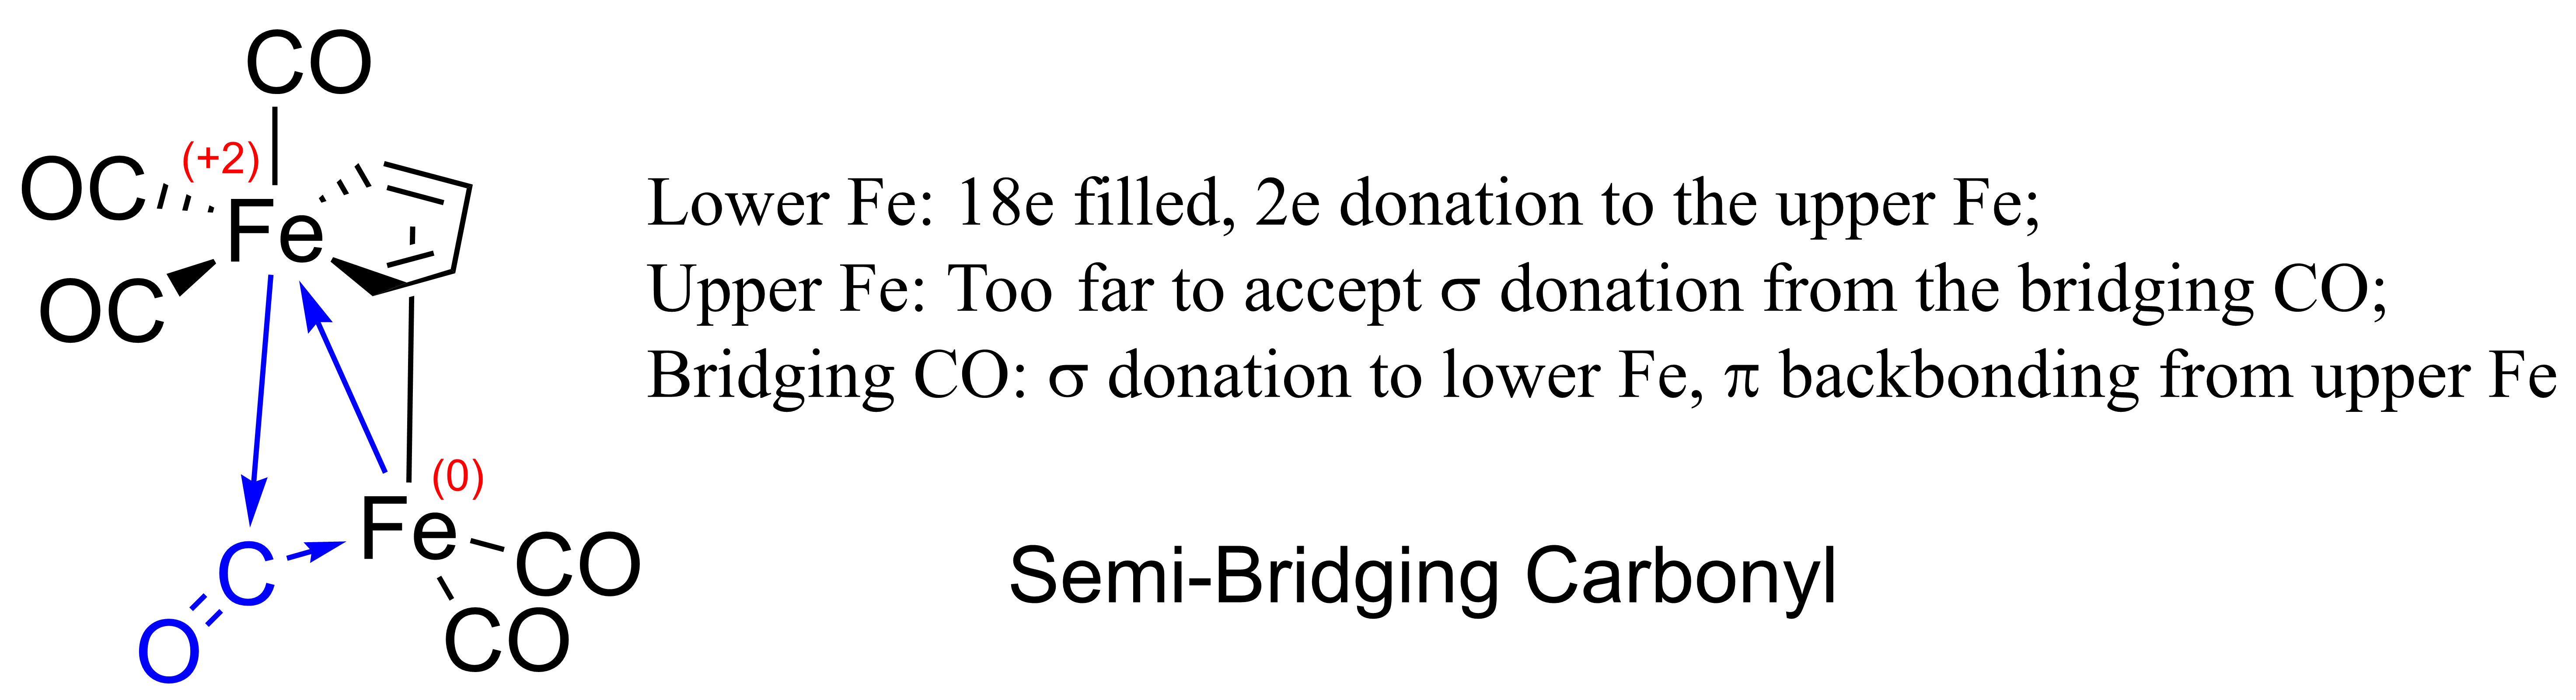
\includegraphics[scale=0.06]{Ch9/semiCO}
\caption{A classic complex containing semi-bridging carbonyl}
\label{semiCO}
\end{figure}
%
\subsubsection{Carbonyl Analogues}
%
Several other ligands function as strong $\pi$ acceptors alongside CO:
%
\begin{itemize}
	\item Isocyanides (CNR): Isoelectronic with CO; stronger $\sigma$ donors due to less electronegative N.
	\item Cyanide (CN$^-$): Coordinate with C end, strong $\sigma$ donor, moderate $\pi$ acceptor;
	\item Azide (N$_3^-$): A weaker version of cyanide;
	\item Phosphines (PR$_3$): $\sigma$ donors via the P lone pair; $\pi$ acceptors through P--R $\sigma^*$ orbitals;
	\item Dinitrogen (N$_2$): Isoelectronic with CO but much weaker due to nonpolarity.
\end{itemize}
%
\subsubsection{Nitrosyl: A Special Case}
%
NO is a radical with one more electron than CO,
giving rise to three coordination modes depending on the metal's electron richness and results in different oxidation states:
%
\begin{enumerate}
	\item Linear NO$^+$: Isoelectronic with CO; M--N--O $\approx 180^\circ$; favored by electron-rich metals.
	\item Bent NO$^\bullet$: M--N--O $\approx 150^\circ$.
	\item Bent NO$^-$: M--N--O $\approx 120$--$130^\circ$; favored by electron-poor metals.
\end{enumerate}
%
\subsection{Pi Complexes with Simple Alkenes}
%
Alkenes coordinate through donation of their $\pi$ bonding pair into an empty metal orbital
and back-donation from a filled metal $d$ orbital into the alkene $\pi^*$ as shown in figure \ref{alkene}
This is the same synergic model as for CO, but with a C=C $\pi$ bond replacing the carbon lone pair.\\
\begin{figure}[h]
\centering
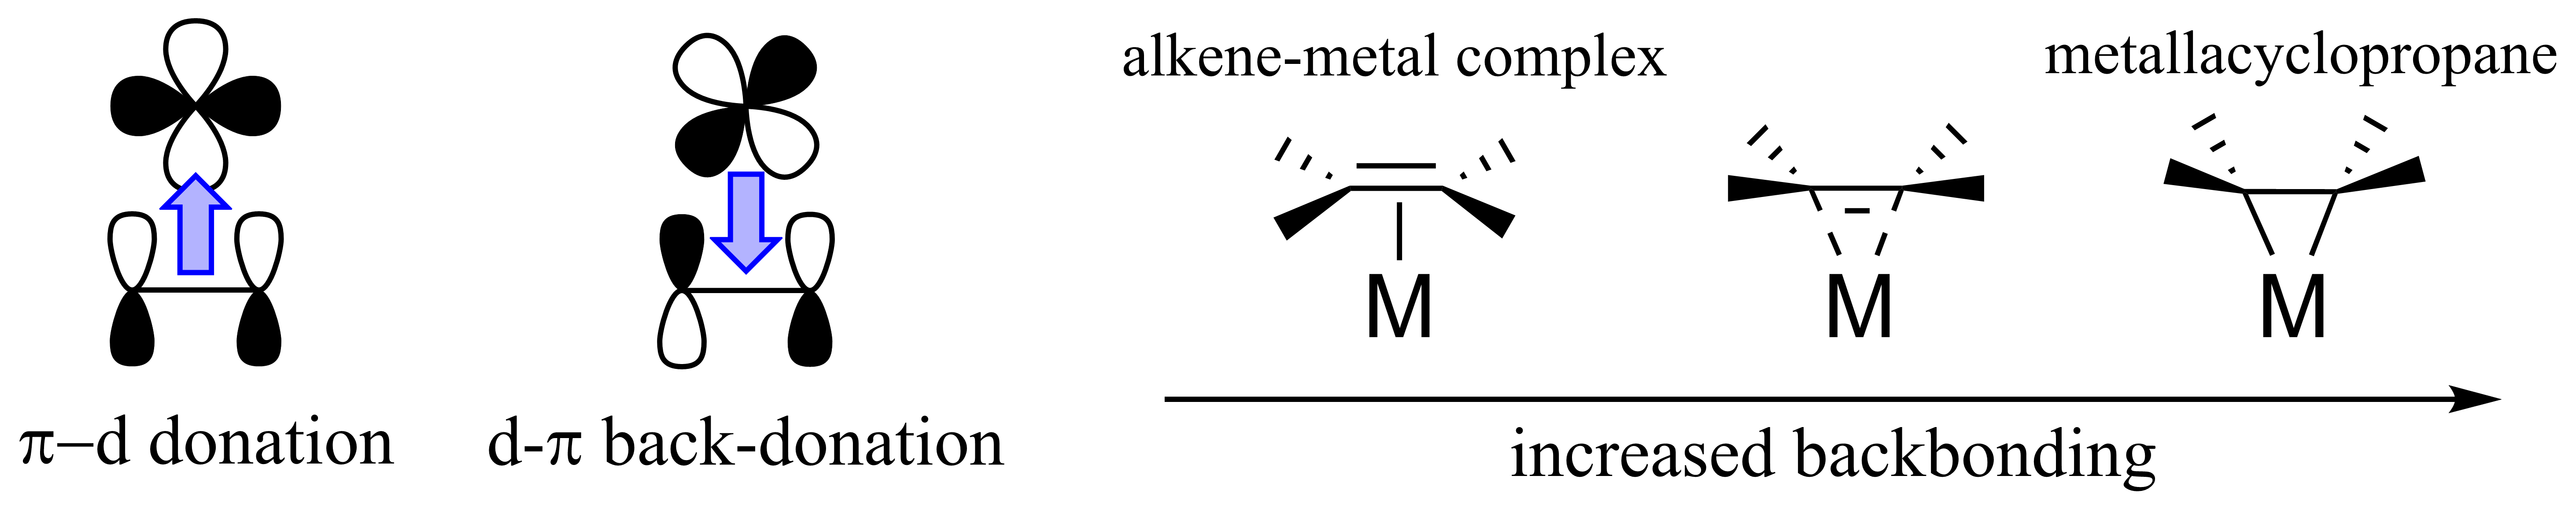
\includegraphics[scale=0.08]{Ch9/alkenemetal}
\caption{Orbital interaction of alkene $\pi$ complexes}
\label{alkene}
\end{figure}\\
%
The degree of back-donation determines where the complex lies on a continuum:
%
\begin{itemize}
	\item \emph{Weak $\pi$ complex}: Minimal back-donation; C=C bond largely intact; substituents planar.
	\item \emph{Metallacyclopropane}: Strong back-donation populates $\pi^*$, lengthening C=C
		and bending substituents back towards the metal.
\end{itemize}
%
Electron-rich metals (low oxidation state, donor co-ligands) favor metallacyclopropane character;
electron-poor metals favor weak $\pi$-complex character.\\ \\
%
Alkynes behave similarly but possess two orthogonal $\pi$ systems,
allowing them to serve as 2e or 4e donors depending on the metal's demand.
In the 4e-donor limit the alkyne bends significantly, approaching metallacyclopropene character.
%
\subsubsection{Dihydrogen and Agostic Complexes}
%
The H--H $\sigma$ bond can itself act as a ligand.
In \emph{dihydrogen complexes} ($\eta^2$-H$_2$), the $\sigma$ bonding pair donates into an empty metal orbital
while metal $d$ electrons back-donate into the $\sigma^*$.
When back-donation suffices to cleave H--H, a \emph{dihydride} results.
The H$_2$ $\rightleftharpoons$ 2H continuum is the $\sigma$-bond analogue of the
$\pi$-complex $\rightleftharpoons$ metallacyclopropane continuum.\\ \\
%
A C--H $\sigma$ bond can similarly coordinate to a metal in an \emph{agostic interaction} 
with orbital interaction pretty much like dihydrogen complexes, which are common in electron-deficient alkyls 
where a low-lying $\sigma^*$ is present.
A three-center two-electron M$\cdots$H--C bond recognized by short M$\cdots$H distances ($\sim$1.8--2.3 \AA)
and red-shifted $\nu_{\text{C--H}}$.
%
\subsubsection{Non-Conjugated Polyenes}
%
Non-conjugated dienes such as 1,5-cyclooctadiene (COD) or norbornadiene
chelate through two independent $\eta^2$ interactions, acting as bidentate L$_2$ ligands.
Each double bond is a separate 2e donor, and the chelate effect provides extra stability.
These ligands are widely used as labile placeholders that are easily displaced during catalysis.
%
\subsection{Pi Complexes with Larger Conjugated Systems}
%
As the conjugated $\pi$ system grows, the elevation of HOMO and supression of LUMO enables better coordination, and
the number of carbons bonded to the metal---the \emph{hapticity}, $\eta^n$---can vary.
Changes in hapticity are a common mechanism for opening coordination sites during catalytic turnover.
%
\subsubsection{Allyl ($\eta^3$-C$_3$H$_5$)}
%
The allyl ligand interconverts between $\eta^1$ ($\sigma$, X-type) and $\eta^3$ ($\pi$, LX-type).
In $\eta^3$ mode, all three carbons interact with the metal through a delocalized $\pi$ system.
The $\eta^1 \rightleftharpoons \eta^3$ equilibrium is central to allylic substitution catalysis:
nucleophilic attack on the $\eta^3$-allyl occurs at the terminal carbons with well-defined stereochemistry.\\ \\
%
Allyl complexes are easily synthesized via allyl substrates with a leaving group (e.g. allyl halides),
as a first alkene coordination promotes the oxidative addition to C--X bond with inversion of configuration.
Also see Tsuji-Trost reaction.
%
\subsubsection{Cyclopentadienyl ($\eta^5$-C$_5$H$_5$)}
%
The cyclopentadienyl (Cp) ligand donates 5 electrons in its $\eta^5$ mode (L$_2$X)
and serves as a robust, spectator-like ligand.
Ferrocene [Fe($\eta^5$-C$_5$H$_5$)$_2$] is the archetype of metallocene chemistry.\\
%
Cp can adopt lower hapticities ($\eta^3$, 3e; $\eta^1$, 1e), especially when coordinated to main group metals.
\emph{Ring slippage} $\eta^5 \to \eta^3 \to \eta^1$ transiently frees a coordination site
while preserving the overall electron count,
a strategy widely exploited in Cp-based catalysis.
%
\subsubsection{Other Cyclic and Open-Chain Polyenes}
%
Other cyclic polyenes as the aromatic benzene and tropylium can coordinate to metals in similar ways, 
even the antiaromatic cyclobutadiene and cyclooctatetraene can be stabilized by back-donation to $\pi^*$.\\ \\
%
The open-chain analogues---\emph{pentadienyl} (C$_5$H$_7$), \emph{heptatrienyl} (C$_7$H$_9$),
and \emph{octatetraenyl} (C$_8$H$_{10}$)---behave similarly to their cyclic counterparts
but with greater conformational flexibility, allowing them to fold around the metal.
In all cases, the metal stabilizes the $\pi$ system, and the hapticity adjusts to satisfy the 18-electron rule.
%
\subsection{Multiple Bonds}
%
Metal--ligand multiple bonds consist of one $\sigma$ bond plus one or more $\pi$ bonds.
They are classified by the number of covalent bond pairs: double (M=X) and triple (M$\equiv$X),
corresponding to X$_2$ and X$_3$ types in the CBC framework.
%
\subsubsection{Oxo, Imido, and Nitrido Complexes}
%
\begin{itemize}
	\item \textbf{Oxo (M=O)}: X$_2$; prevalent in high-valent early metals (e.g.\ d$^0$ [MoO$_2$Cl$_2$]).
		Strong O $\pi$ donation raises the metal $t_{2g}$-like orbitals,
		making terminal oxo groups rare in electron-rich late metals.
	\item \textbf{Imido (M=NR)}: X$_2$; the R substituent provides tunability.
		Can be linear (maximal $\pi$ overlap) or bent (reduced $\pi$ donation)
		depending on the metal's electron demand.
	\item \textbf{Nitrido (M$\equiv$N)}: X$_3$; N donates three electrons.
		Requires an electron-poor metal in a high oxidation state capable of accepting three $\pi$ donations.
\end{itemize}
%
\subsubsection{Alkylidene and Alkylidyne Complexes}
%
Carbene (alkylidene, M=CR$_2$, X$_2$) and carbyne (alkylidyne, M$\equiv$CR, X$_3$) complexes
feature metal--carbon multiple bonds and are among the most important ligands in modern catalysis.
%
\subsubsection{Fischer vs.\ Schrock Carbenes}
%
Metal carbenes fall into two classes based on their electronic structure and reactivity:
%
\begin{itemize}
	\item \textbf{Fischer carbenes}: Low-oxidation-state metal with $\pi$-acceptor co-ligands (e.g.\ CO).
		The carbene carbon is \emph{electrophilic}.
		Bonding is best described as a singlet carbene ($sp^2$, vacant $p$ orbital) interacting with the metal:
		strong $\sigma$ donation from C, moderate $\pi$ back-donation from the metal.
		Reacts with nucleophiles.
	\item \textbf{Schrock carbenes}: High-oxidation-state metal with $\sigma$-donor co-ligands (e.g.\ alkyl, Cp).
		The carbene carbon is \emph{nucleophilic}.
		Bonding is best described as a triplet carbene (two singly occupied orbitals) interacting with the metal:
		covalent $\sigma$ and $\pi$ bonds formed by electron pairing.
		Reacts with electrophiles; key intermediates in olefin metathesis (Schrock and Grubbs catalysts).
\end{itemize}
%
The distinction maps onto the singlet/triplet state of the free carbene:
Fischer carbenes are metal-stabilized singlet carbenes, while Schrock carbenes are metal-stabilized triplet carbenes.
%
\subsection{Inverse Coordination}
%
In conventional coordination chemistry, the metal acts as the electron acceptor
and the frontier orbitals (HOMO/LUMO) are metal $d$ in character.
However, when ligands possess exceptionally strong $\sigma$-donor character,
the direction of charge transfer can be effectively reversed:
electron density flows so completely from ligands to metal that
the frontier orbitals of the resulting complex become ligand-dominated rather than metal-dominated.\\
\begin{figure}[h]
\centering
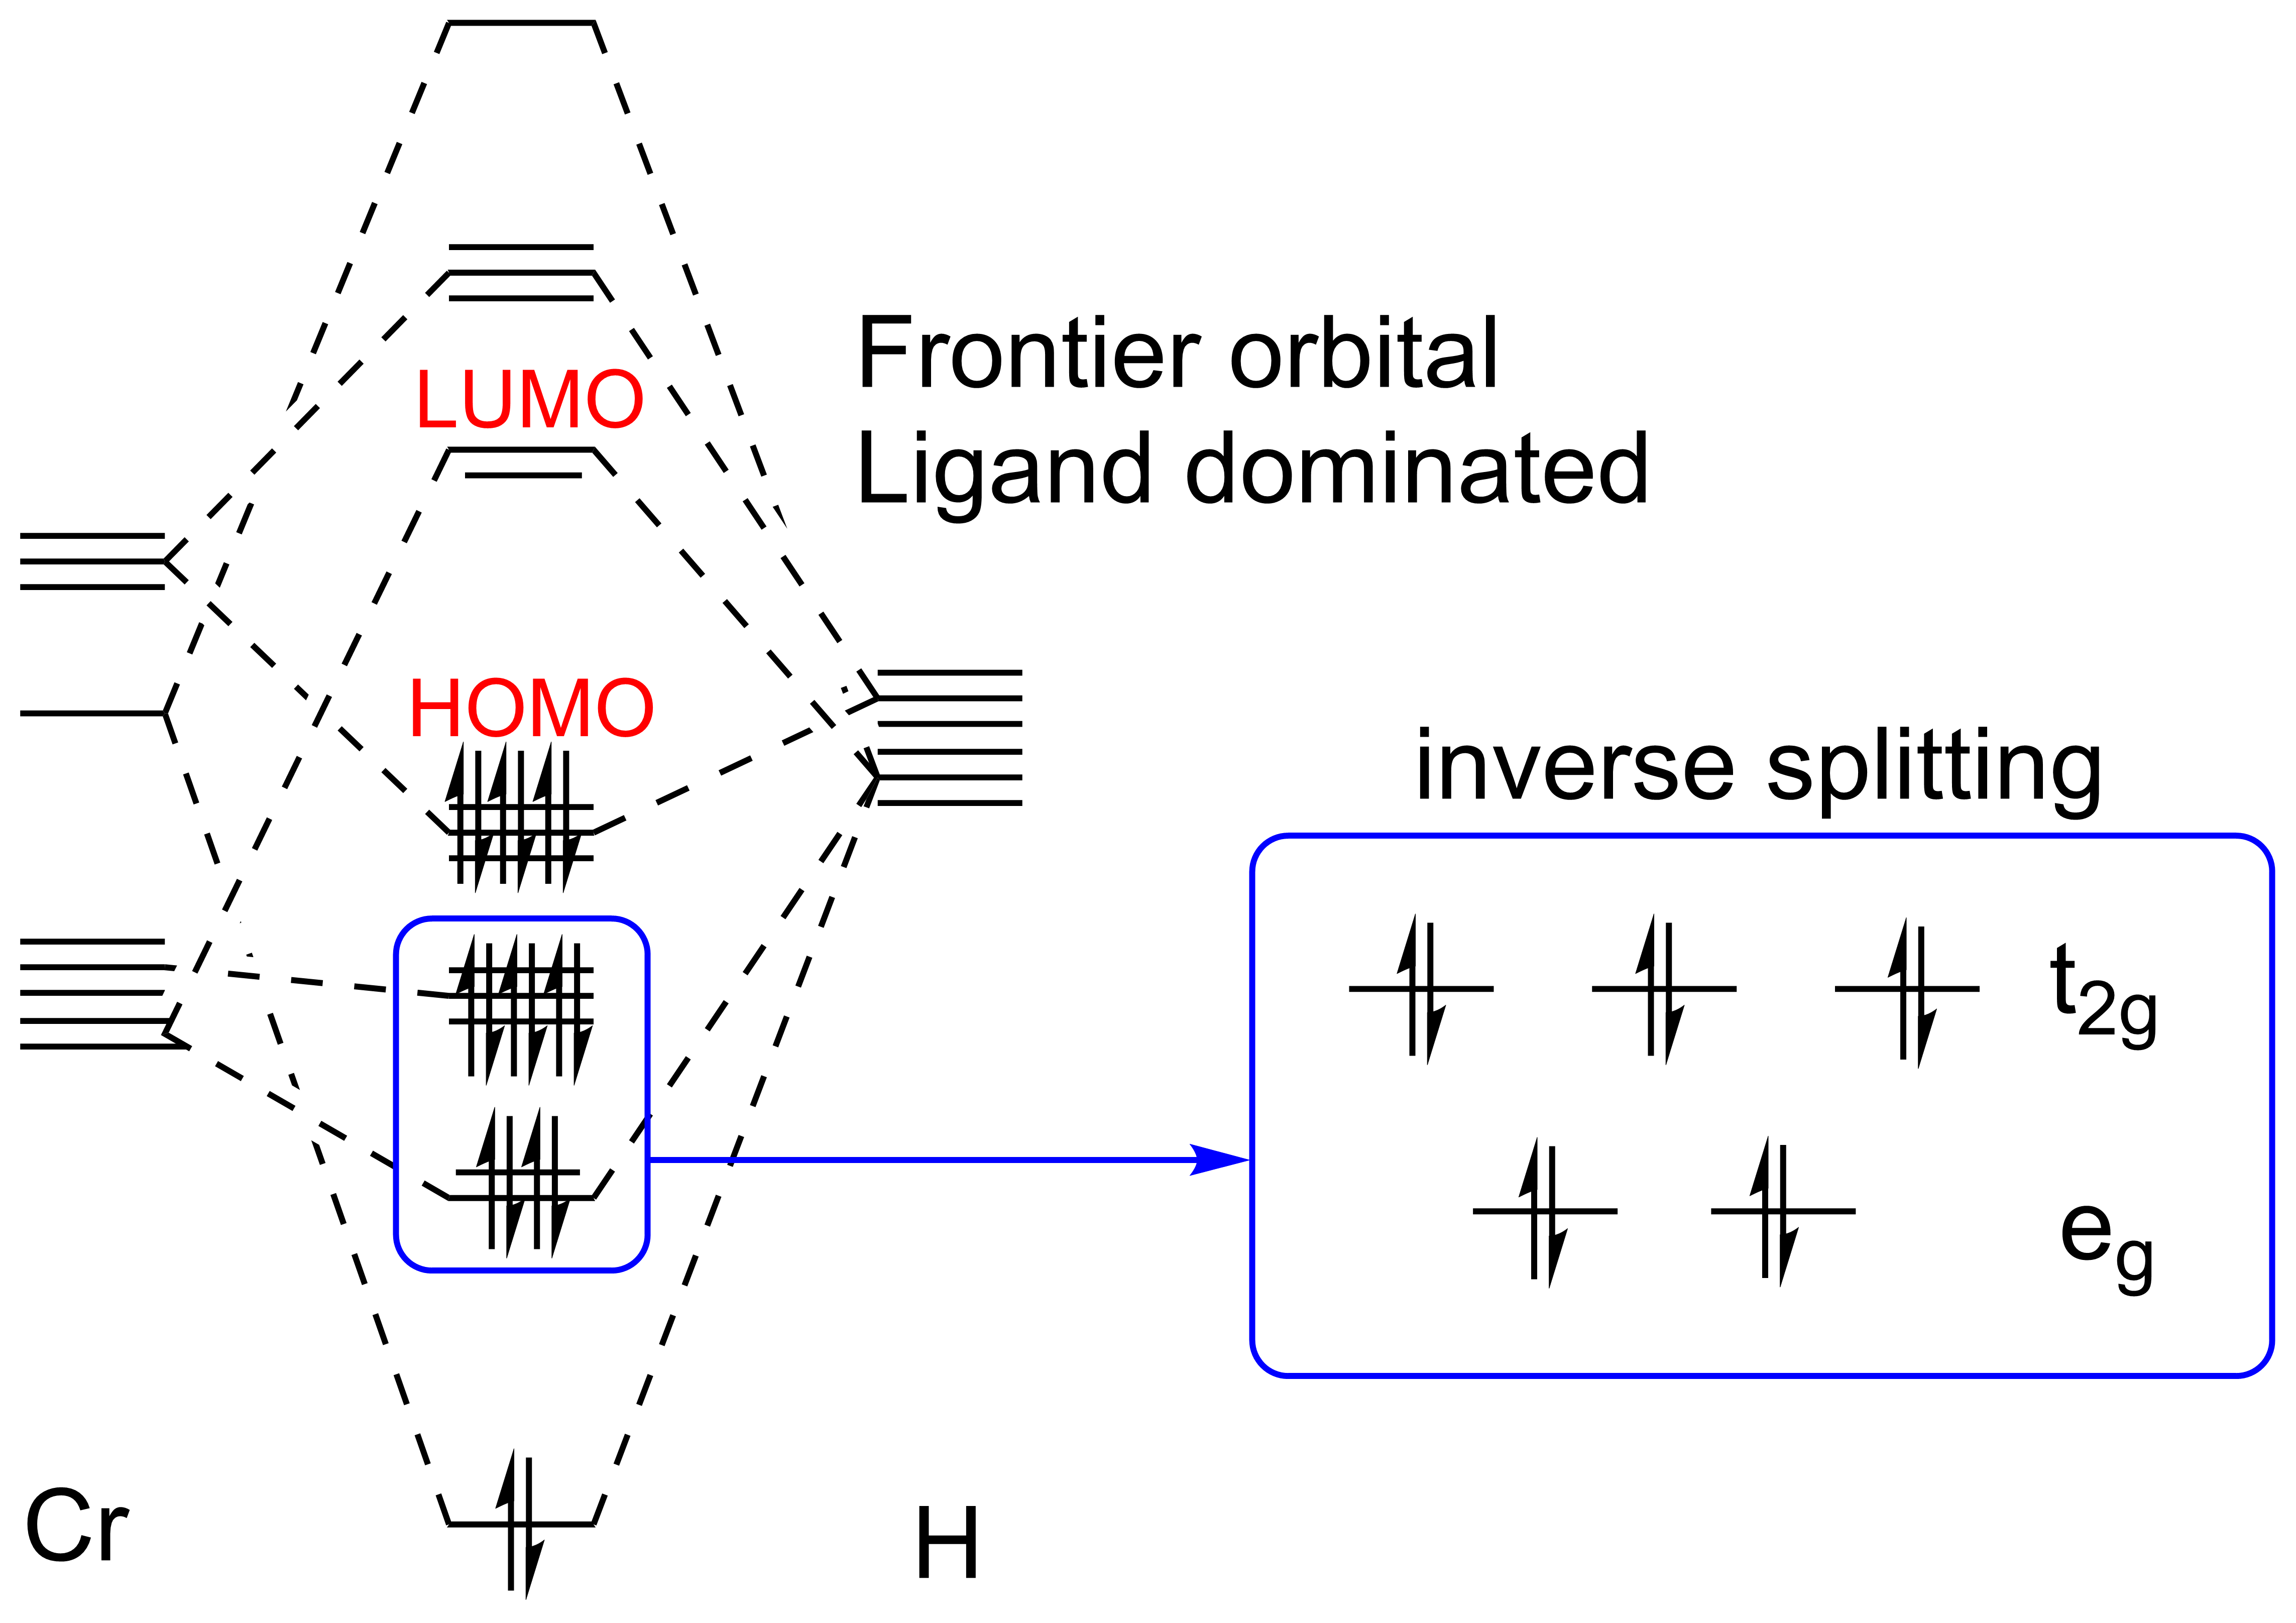
\includegraphics[scale=0.06]{Ch9/inverse}
\caption{Orbital profile of $[\text{CrH}_6]^{6-}$}
\label{inverse}
\end{figure}\\
%
A classic example is $[\text{CrH}_6]^{6-}$, where six hydride ligands donate so strongly
that the HOMO and LUMO are both ligand-centered SALCs, shown in figure \ref{inverse}.
The metal $d$ orbitals are pushed to higher energy and no longer define the frontier.
The metal effectively becomes a ``pseudo-anion'' embedded in a ligand-dominated orbital manifold.\\ \\
%
This phenomenon, termed \emph{inverse coordination},
represents the extreme limit of the ligand-field picture discussed in \ref{split}:
when $\sigma$ donation overwhelms the metal's ability to accept electron density,
the usual ordering in which metal $t_{2g}$ orbitals lie between bonding and antibonding ligand orbitals is inverted,
and the complex's reactivity is governed by ligand-based rather than metal-based orbitals.
%
\subsection{Trans Effect}
For square planar and octahedral complexes, two coordination sites are in trans position if they are symmetric about $i$ (inversion).
As $d$ orbitals are all inversion-symmetrical, ligands on one site will have a significant impact on its trans position, 
weakening coordination bond and fostering ligand substitution. 
\begin{itemize}
\item \textbf{Strong $\sigma$ bases} as H$^-$ or CH$_3^-$: Strong electron donation increases $d$ orbital electron density, 
leading to a polarized elongation along bonding axis, filling the ligand-metal $\sigma^*$ orbital of the trans position and thus weaken the bond.
\item \textbf{Strong $\pi$ acids} as CO or CN$^-$: strong electron withdrawing effect sucks up the electron density the trans ligand donates to the metal, 
decreasing the covalent character of the M--L bond and thus weakening the bond.
\end{itemize}